\documentclass[10pt,a4paper]{article}
\usepackage{fullpage}
\usepackage{booktabs}
\usepackage{amsmath}
\usepackage{graphicx}
\usepackage{todonotes}
\usepackage{multirow,matlab-prettifier}
\usepackage[T1]{fontenc}

\hyphenpenalty=5000
\tolerance=1000

\newcommand{\qmax}[0]{Q_{\textrm{max}}}
\newcommand{\nuab}[0]{$\nu_{ab}$}

\newcommand{\nuee}[0]{$\nu_{ee}$}
\newcommand{\nuei}[0]{$\nu_{ei}$}
\newcommand{\nues}[0]{$\nu_{es}$}
\newcommand{\nuse}[0]{$\nu_{se}$}
\newcommand{\nusr}[0]{$\nu_{sr}$}
\newcommand{\nusn}[0]{$\nu_{sn}$}
\newcommand{\nure}[0]{$\nu_{re}$}
\newcommand{\nurs}[0]{$\nu_{rs}$}

\newcommand{\gab}[0]{$G_{ab}$}

\newcommand{\gabcd}[0]{$G_{abcd}$}
\newcommand{\gese}[0]{$G_{ese}$}
\newcommand{\gesre}[0]{$G_{esre}$}
\newcommand{\gsrs}[0]{$G_{srs}$}

\newcommand{\xyz}[0]{$XY\!Z$}

\newcommand{\gee}[0]{$G_{ee}$}
\newcommand{\gei}[0]{$G_{ei}$}
\newcommand{\ges}[0]{$G_{es}$}
\newcommand{\gse}[0]{$G_{se}$}
\newcommand{\gsr}[0]{$G_{sr}$}
\newcommand{\gsn}[0]{$G_{sn}$}
\newcommand{\gre}[0]{$G_{re}$}
\newcommand{\grs}[0]{$G_{rs}$}
\newcommand{\e}[1]{\times 10^{#1}}
\newcommand{\phia}[0]{$\phi_a$}
\newcommand{\phie}[0]{$\phi_e$}
\newcommand{\phii}[0]{$\phi_i$}
\newcommand{\phir}[0]{$\phi_r$}	
\newcommand{\phis}[0]{$\phi_s$}
\newcommand{\phies}[0]{$\phi_{es}$}
\newcommand{\phirs}[0]{$\phi_{rs}$}
\newcommand{\phin}[0]{$\phi_n$}
\newcommand{\vsnl}[0]{$V^{(2)}_s(\mathbf{k},\omega)$}

\usepackage{setspace}
\onehalfspacing

\begin{document}

\section{MCMC Alternate Models}
{\bf Romesh Abeysuriya} \today
\sffamily

This document outlines the different models available for the MCMC fitting. In terms of code, {\tt template.m} is the abstract class that provides the standard interface for all model objects. 

\begin{align}
\mathcal{F}(D_\alpha) &= \left(1 - \frac{i\omega}{\alpha}\right)\left(1 - \frac{i\omega}{\beta}\right)\\[16pt]
\mathcal{F}(D_a) &= \left( 1-\frac{i\omega}{\gamma}\right)^2 + k^2r^2
\end{align}

\subsection{Full model}

Implemented in {\tt full.m}. Includes EMG. 

\begin{figure}[h!]
\begin{center}
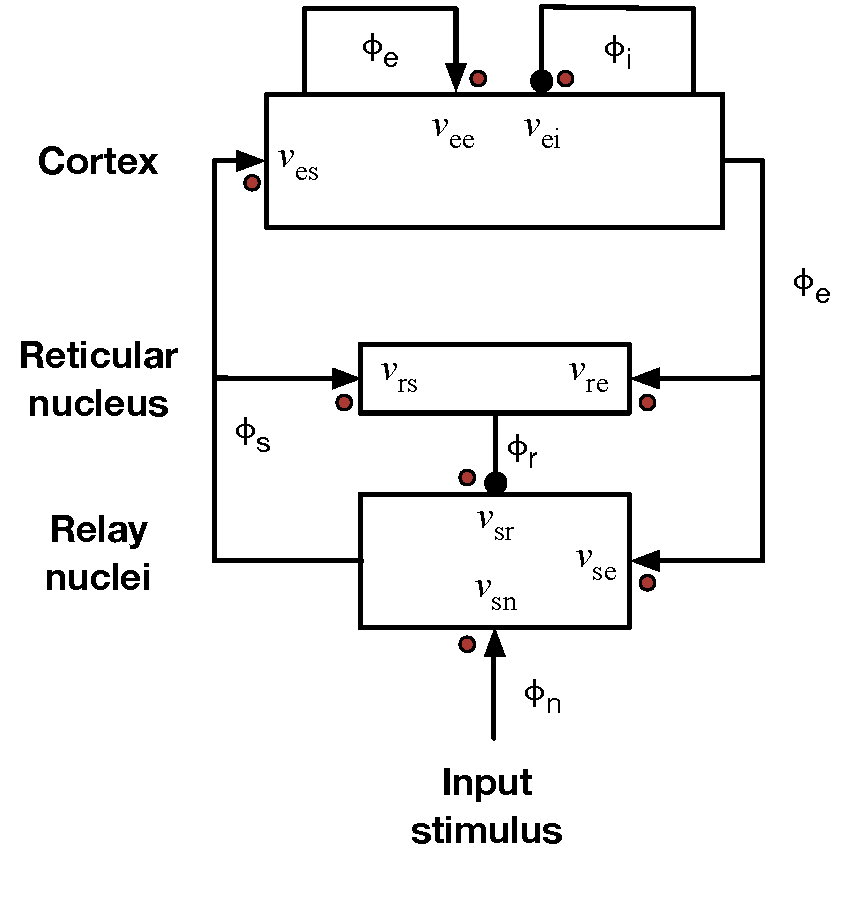
\includegraphics[width=0.4\textwidth]{full_model}
\caption{Full model schematic. A factor of $L$ is included for each connection marked with a red dot.}
\label{fig:full}
\end{center}
\end{figure}

This model implements the full EIRS system, in terms of the gains. Volume condution is incorporated with

\begin{align}
\mathbf{k} &= \left( \frac{2\pi m}{L_x},\frac{2\pi n}{L_y} \right),\\
F(k) &= e^{-k^2/k_0^2}.
\end{align}

The power spectrum is given by

\begin{align}
 q^2r_e^2 &= \left( 1-\frac{i\omega}{\gamma_e} \right)^2   - \frac{1}{1-G_{ei}L} \left\lbrace LG_{ee} + \frac{\left[ L^2G_{ese}  + L^3 G_{erse}\right]e^{i\omega t_0}}{1 - L^2 G_{srs}}  \right\rbrace \\
T &=  \frac{L^2G_{esn}e^{i\omega t_0 /2}}{(1 - L^2 G_{srs})(1-G_{ei}L)} \frac{1}{k^2r_e^2 + q^2r_e^2}\\
 P(\omega) &= \sum_{m = -\infty}^{\infty}\sum_{n = -\infty}^{\infty} \Delta k_x \Delta k_y |T(\mathbf{k},\omega)|^2||\phi_n(\mathbf{k},\omega)|^2F(k)\\
k^2 &=  \left( \frac{2\pi m}{L_x} \right)^2 + \left( \frac{2\pi n}{L_y}\right)^2 
\end{align}

Stability is identified by negative real part zero crossings of the dispersion relation

\begin{align}
\label{eqn:dispersion_relation}
\left( \left[ \left( 1-\frac{i\omega}{\gamma_e} \right)^2 + k^2r_e^2 \right](1-G_{ei}L) - LG_{ee} \right) (1 - L^2 G_{srs}) - (L^2G_{ese}  + L^3 G_{erse})e^{i\omega t_0} &= 0
\end{align}

\begin{figure}[h!]
\begin{center}
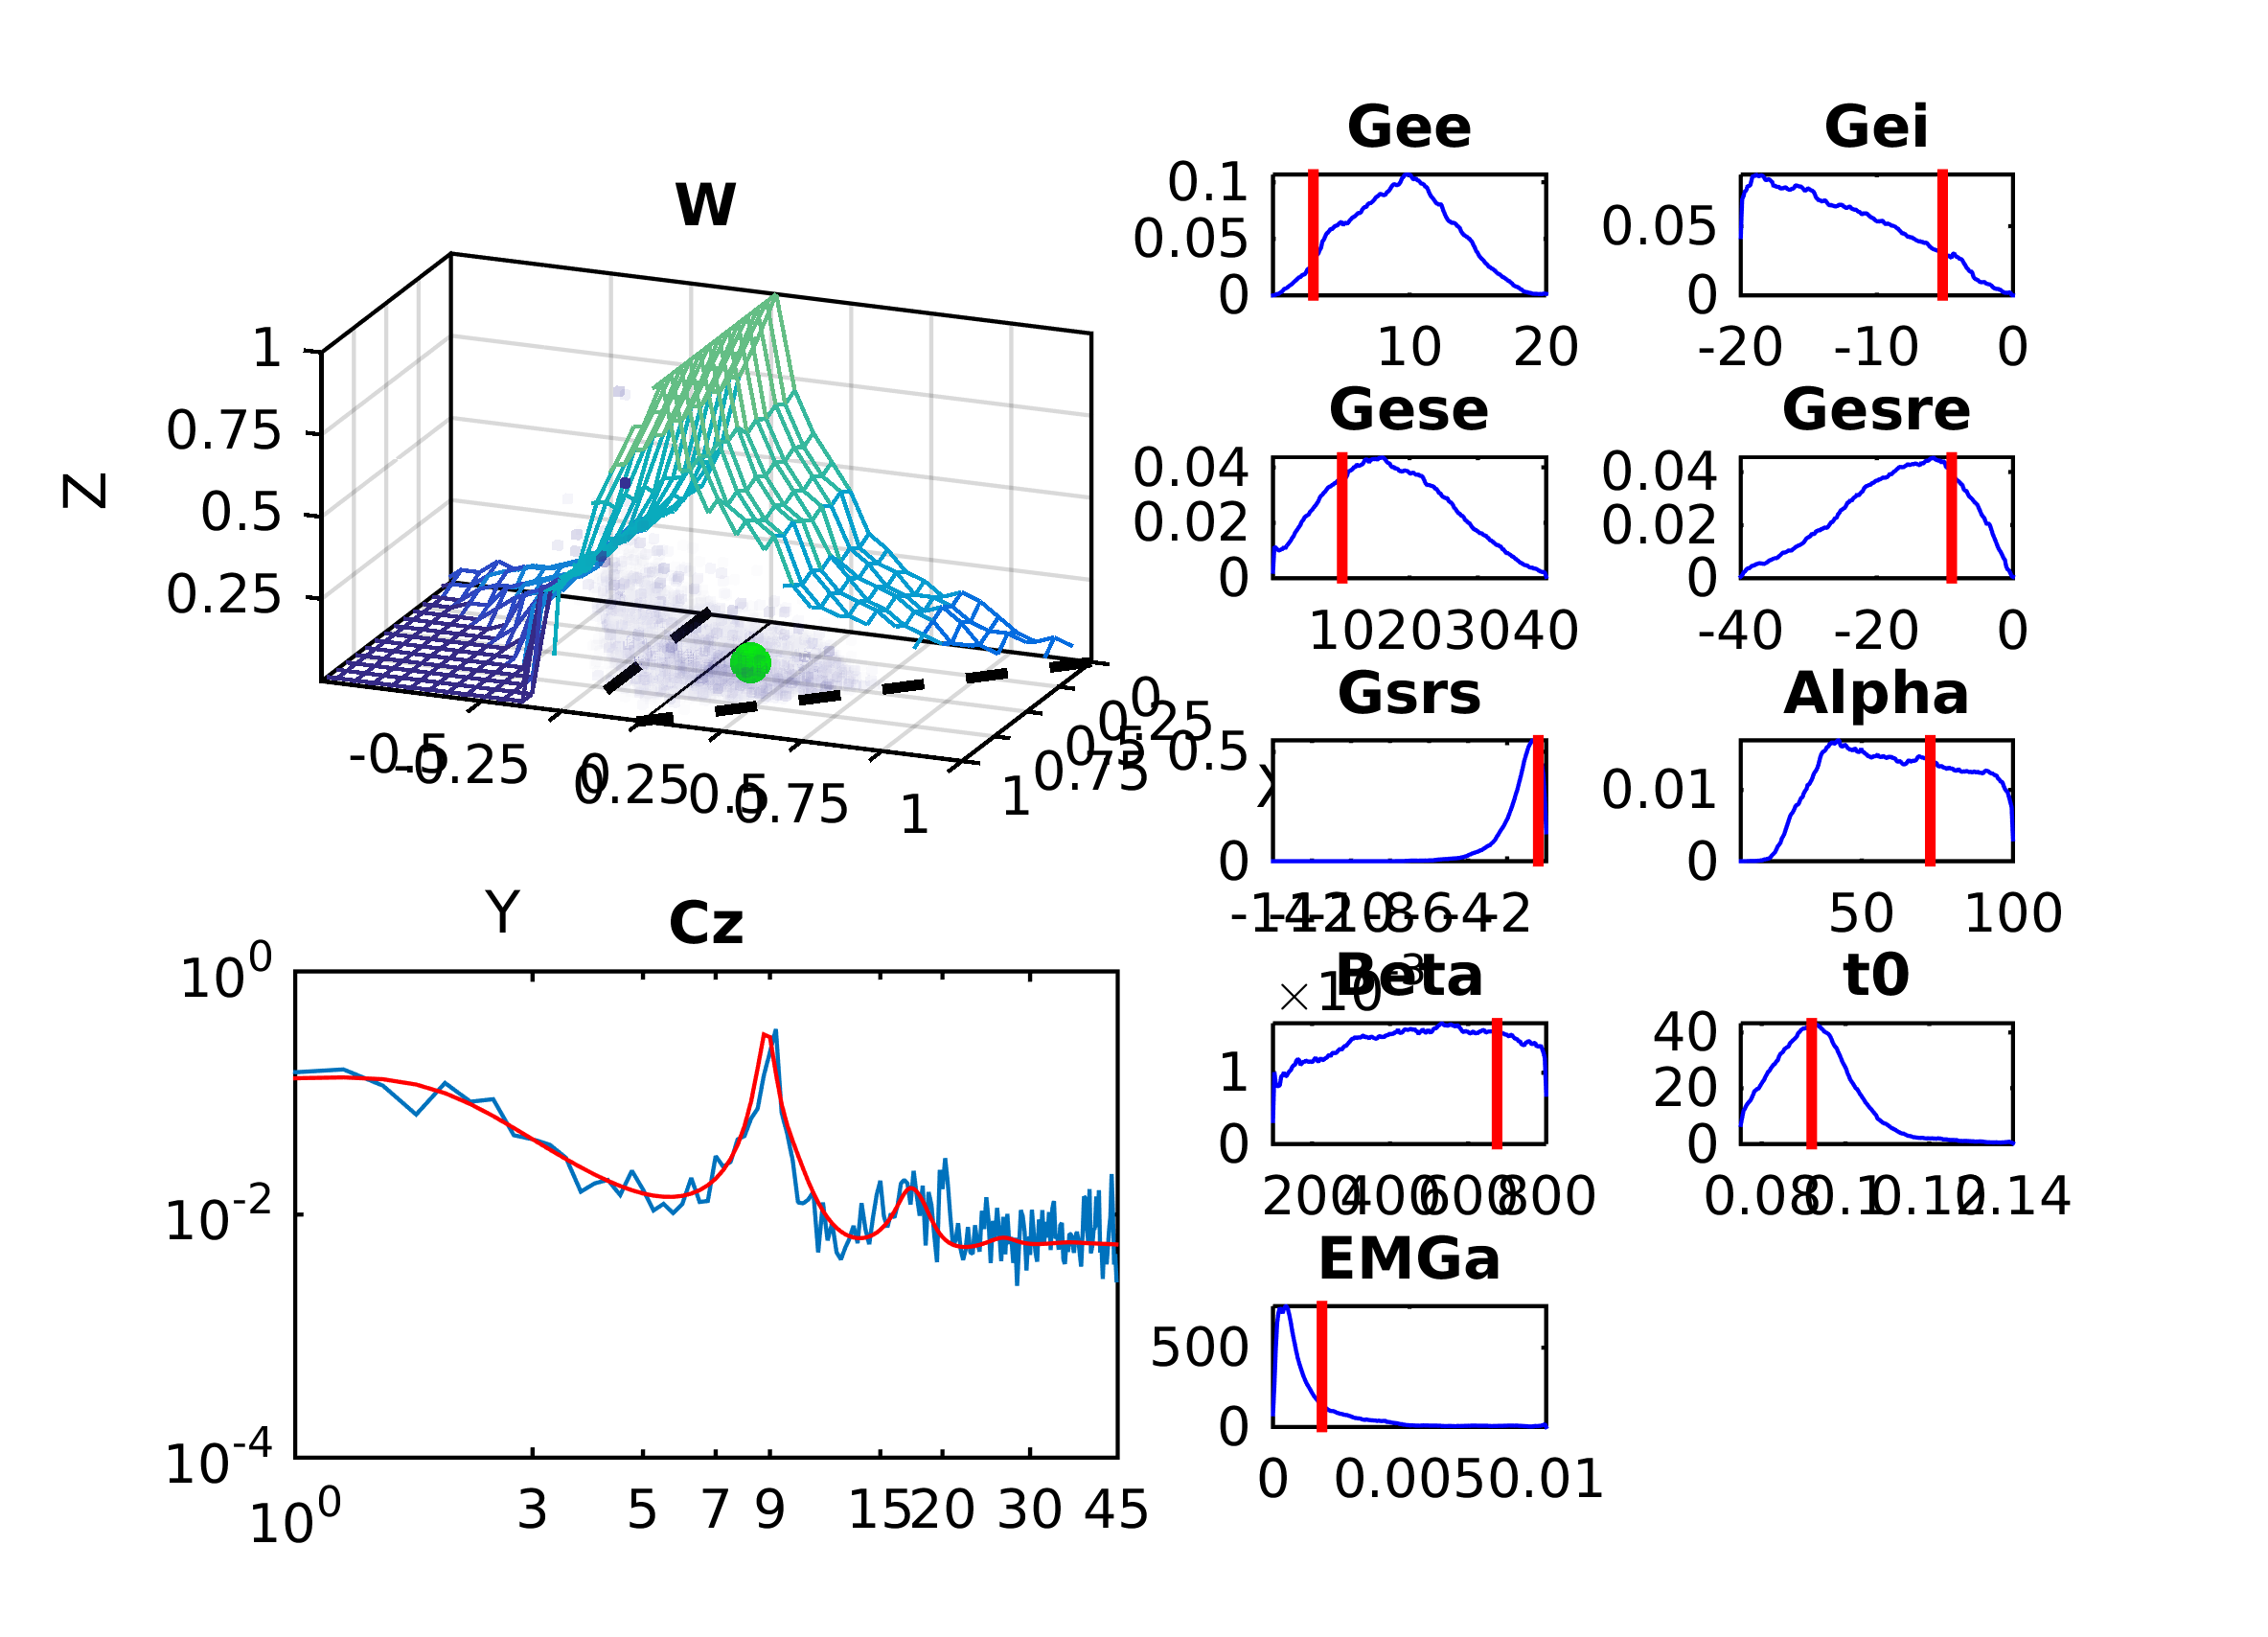
\includegraphics[width=0.8\textwidth]{example_full}
\caption{Example fit with full model.}
\label{fig:full}
\end{center}
\end{figure}

\begin{figure}[h!]
\begin{center}
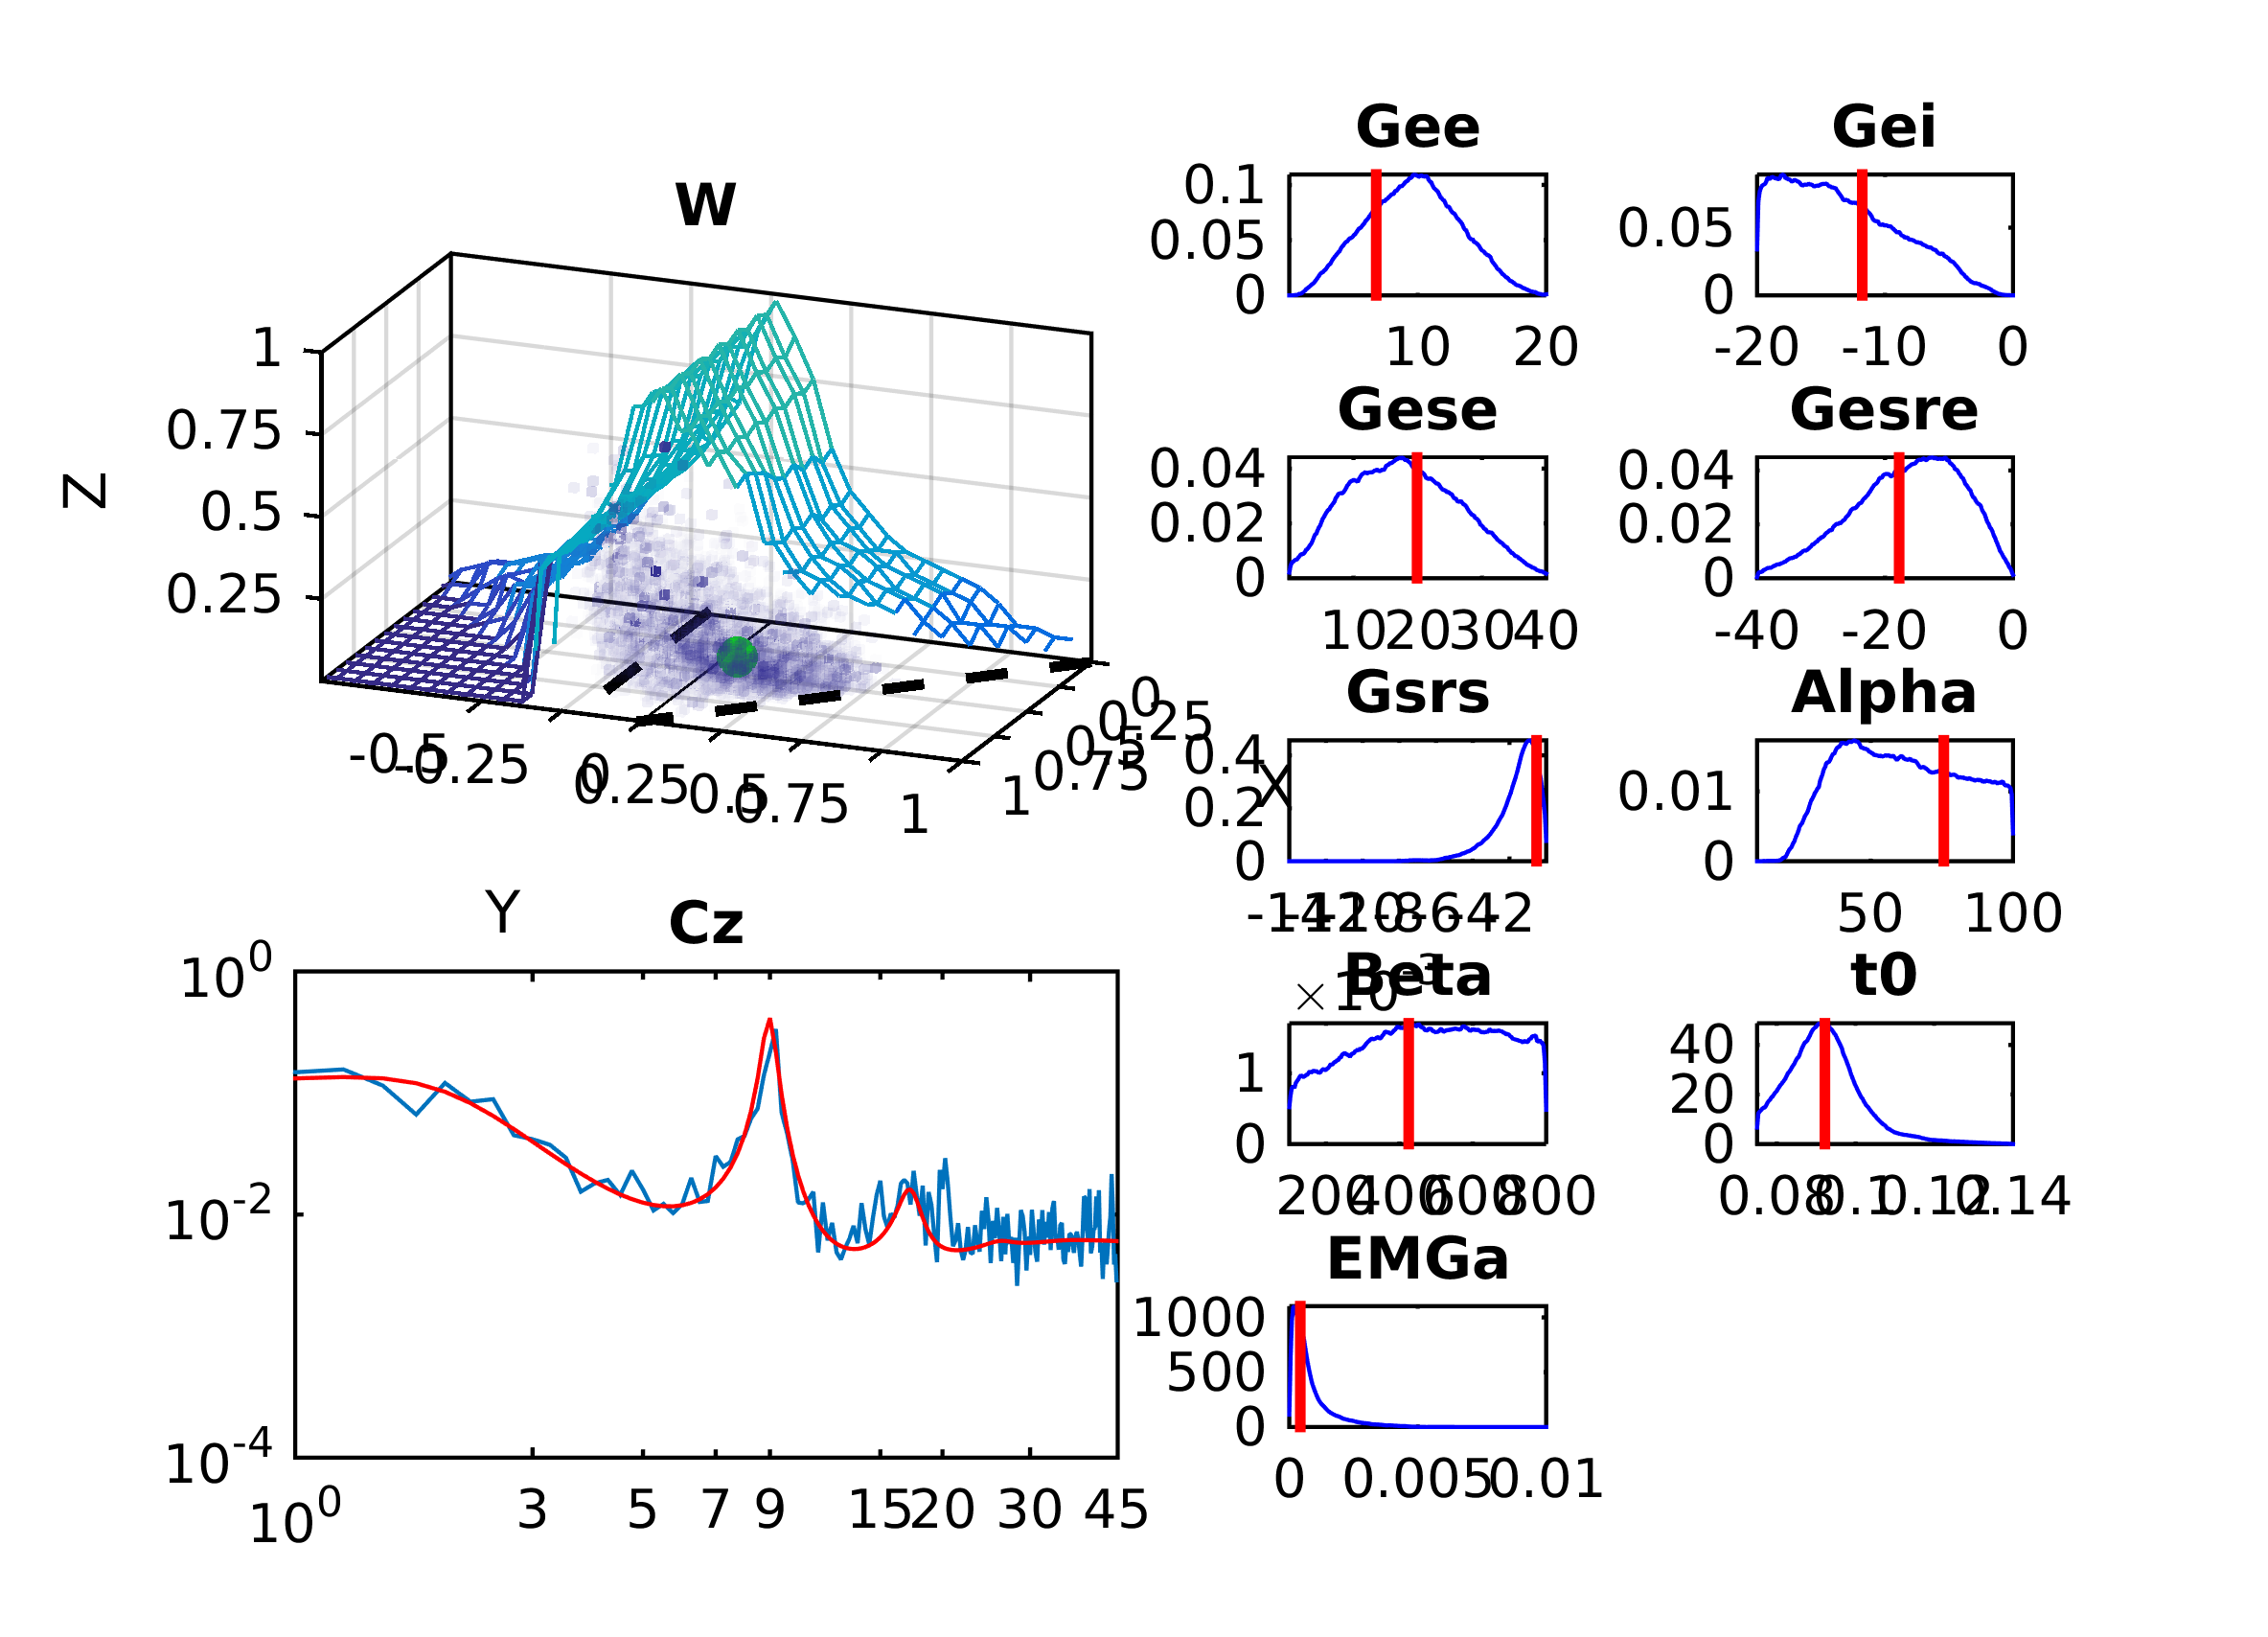
\includegraphics[width=0.8\textwidth]{example_full_k0}
\caption{Example fit with full model, with $k=0$ only.}
\label{fig:full}
\end{center}
\end{figure}

\clearpage

\subsection{Reduced model with L}
Implemented in {\tt reduced\_l.m}. This is a new model, and bears the most (implementation) similarity to the full model. In this model, $L_{sr}$ is moved to the connection $rs$. Thus the $srs$ loop still gets two factors of $L$, but now $L_{ese} = L_{erse}$. This enables factorization of the $L$ terms in $Y$. However, separate parameters are still required for $G_{ee}$ and $G_{ei}$. 

\begin{figure}[h!]
\begin{center}
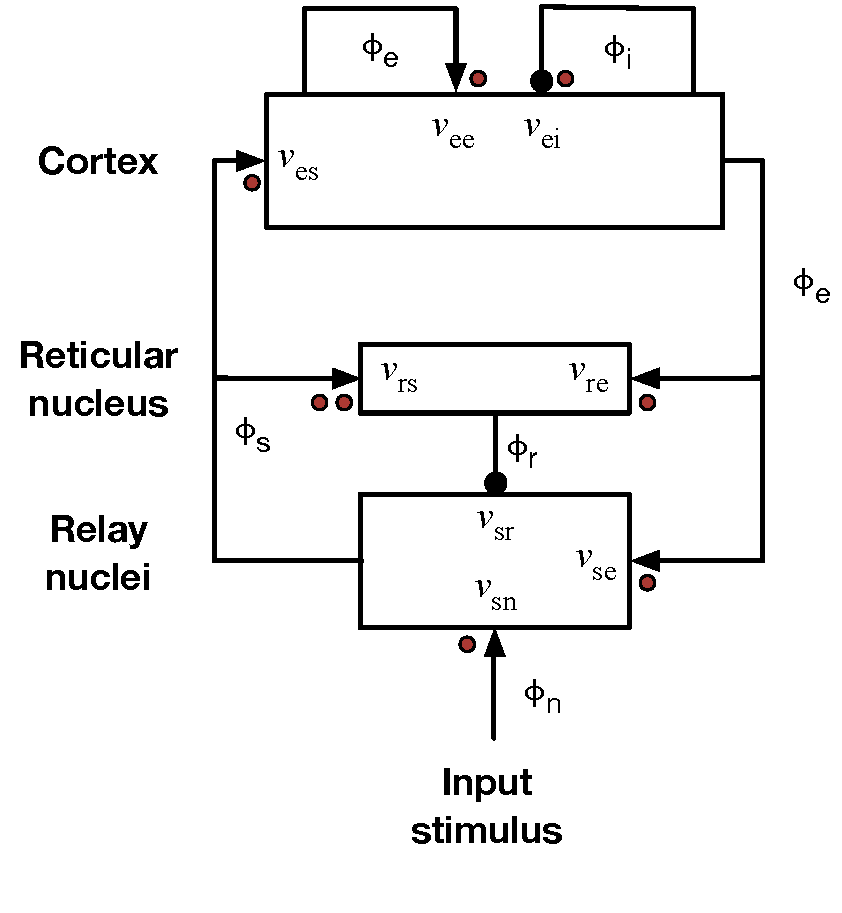
\includegraphics[width=0.4\textwidth]{reduced_l}
\caption{Full model schematic. A factor of $L$ is included for each connection marked with a red dot.}
\label{fig:full}
\end{center}
\end{figure}

The power spectrum is given by

\begin{align}
 q^2r_e^2 &=  \left( 1-\frac{i\omega}{\gamma_e} \right)^2 - \frac{LG_{ee}}{1-LG_{ei}} - \frac{L^2(Y\left( 1+Z'\right)(1-G_{ei}))e^{i\omega t_0}}{\left( 1+Z' L^2 \right)(1-LG_{ei})}\\
 T &=  \frac{L^2G_{esn}e^{i\omega t_0 /2}}{(1 - L^2 G_{srs})(1-G_{ei}L)} \frac{1}{k^2r_e^2 + q^2r_e^2}\\
 P(\omega) &= \sum_{m = -\infty}^{\infty}\sum_{n = -\infty}^{\infty} \Delta k_x \Delta k_y |T(\mathbf{k},\omega)|^2||\phi_n(\mathbf{k},\omega)|^2F(k)\\
k^2 &=  \left( \frac{2\pi m}{L_x} \right)^2 + \left( \frac{2\pi n}{L_y}\right)^2 
\end{align}

Stability is identified by negative real part zero crossings of the dispersion relation

\begin{align}
\label{eqn:dispersion_relation}
\left( \left[ \left( 1-\frac{i\omega}{\gamma_e} \right)^2 + k^2r_e^2 \right](1-G_{ei}L) - LG_{ee} \right) \left( 1+Z' L^2 \right) - L^2 Y\left( 1+Z' \right)\left( 1-G_{ei} \right) e^{i\omega t_0} &= 0
\end{align}

\begin{figure}[h!]
\begin{center}
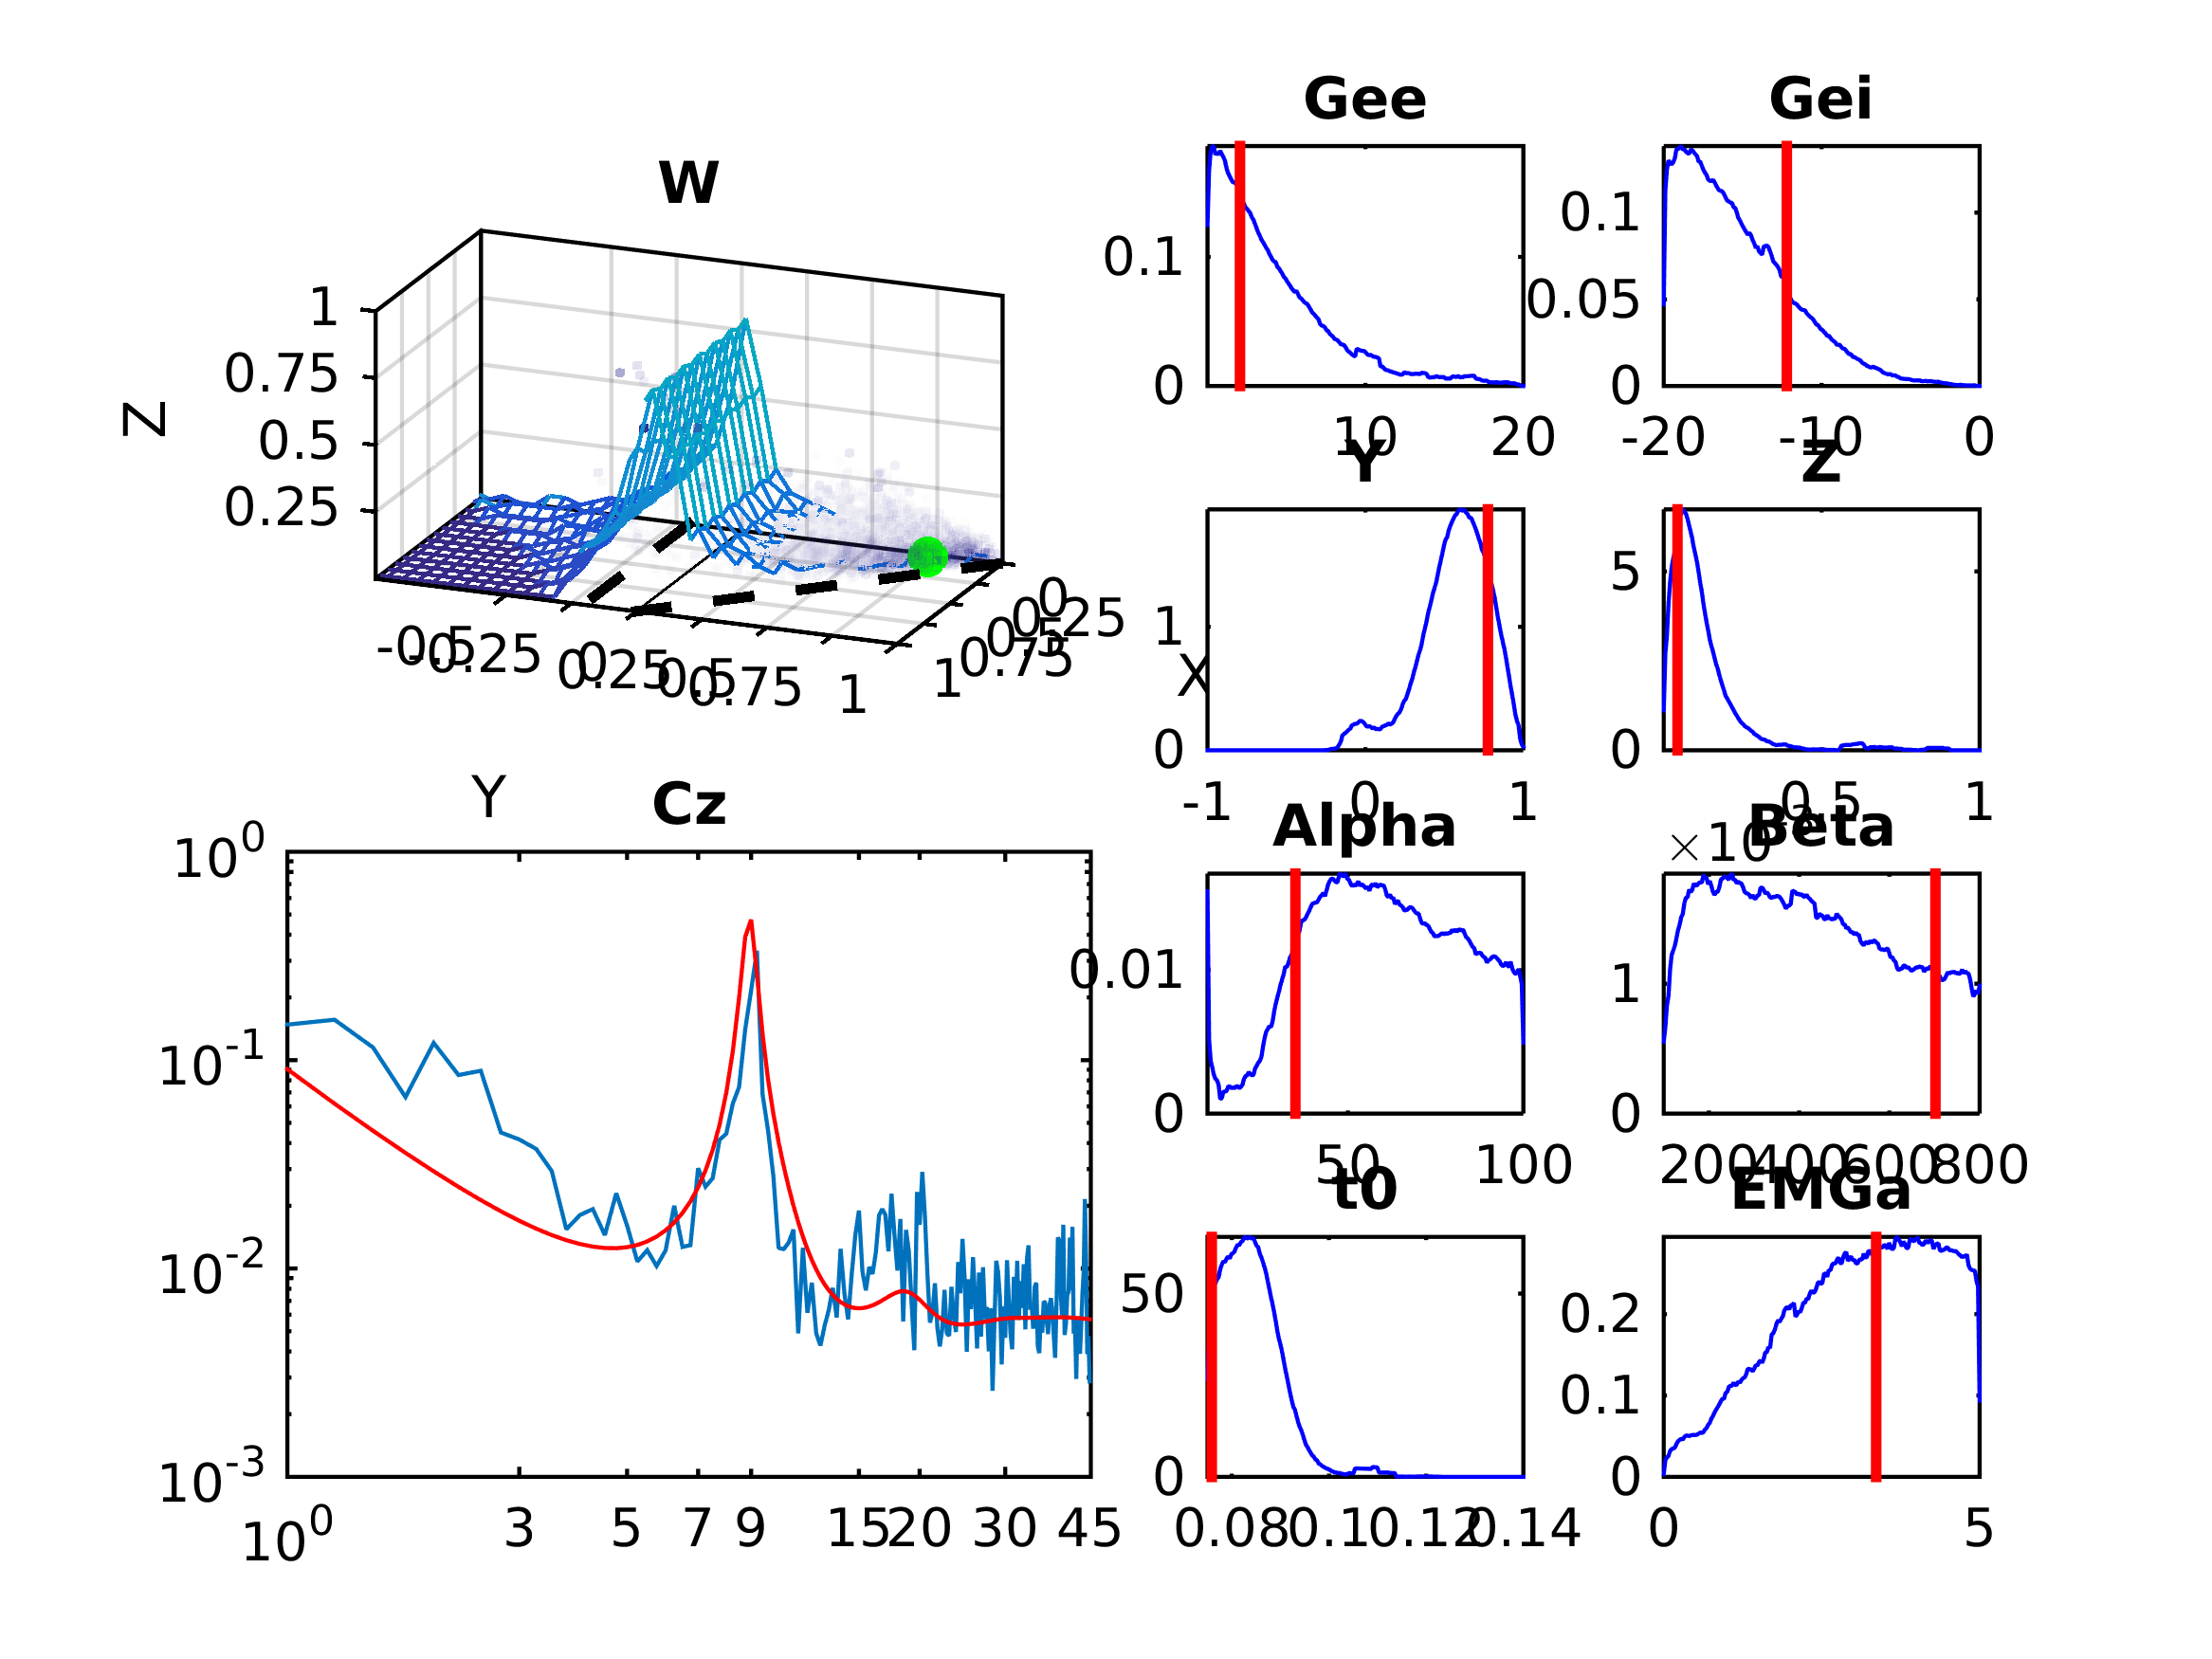
\includegraphics[width=0.8\textwidth]{example_reduced_l}
\caption{Example fit with \texttt{reduced\_l}.}
\label{fig:full}
\end{center}
\end{figure}

\clearpage

\subsection{Reduced model}
Implemented in {\tt reduced.m}

Normal reduced model including EMG. Equations are derived by substituting $L = 1$ into the full model except in $(1-G_{srs}L^2)$. 

\begin{figure}[h!]
\begin{center}
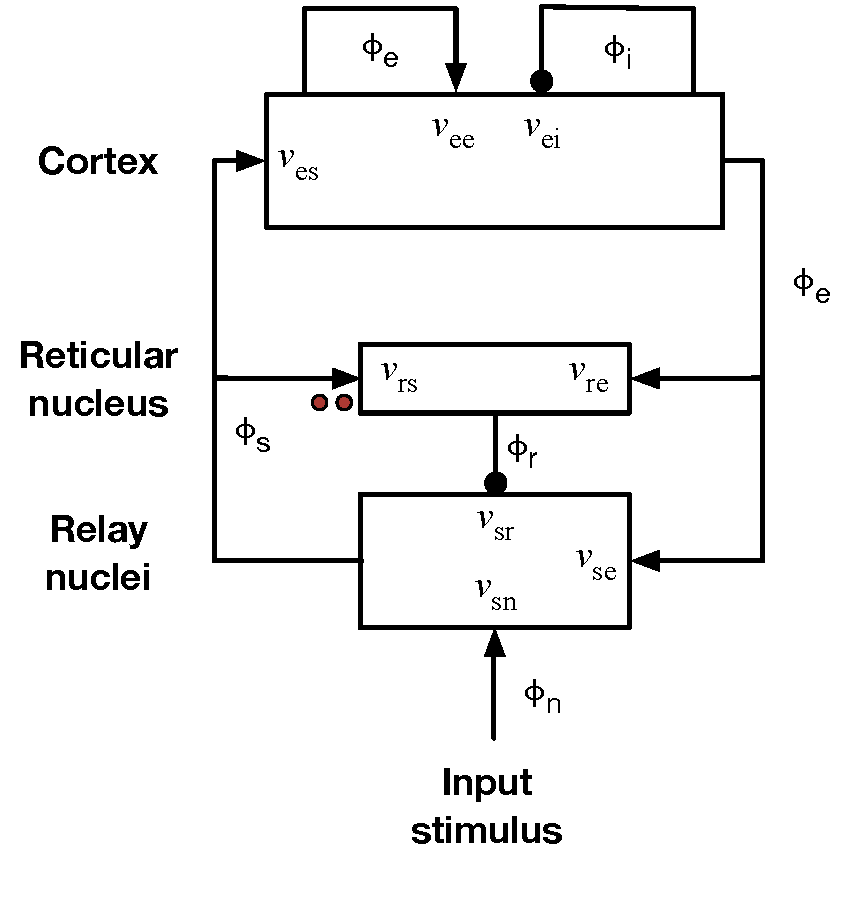
\includegraphics[width=0.4\textwidth]{reduced}
\caption{Reduced model schematic. A factor of $L$ is included for each connection marked with a red dot.}
\label{fig:full}
\end{center}
\end{figure}

Key parameters are $X$, $Y$, $Z$. Stability is given using the dispersion relation
\begin{align}
	\left[ \left(1-\frac{i\omega}{\gamma}\right)^2 - X + k^2r_e^2 \right] \left( 1+Z' L^2 \right) - Y\left( 1+Z' \right) e^{i\omega t_0} &= 0, %JAMES DISPERSION RELATION
\end{align}

with $k=0$. The power spectrum is given by

\begin{align}
	q^2r_e^2 &= \left( 1 - \frac{i \omega}{\gamma}\right)^2  - X - \frac{Y(1+Z')}{1+Z'L^2}e^{i\omega t_0},\\[14pt]
	P(\omega) &= \sum_{m = -\infty}^{\infty}\sum_{n = -\infty}^{\infty} P_0 \left| \frac{1}{(1+Z'L^2)(k^2r_e^2+q^2r_e^2)}\right|^2,\\[14pt]
	Z' &= Z \frac{(\alpha+\beta)^2}{\alpha\beta},
\end{align}

\begin{figure}[h!]
\begin{center}
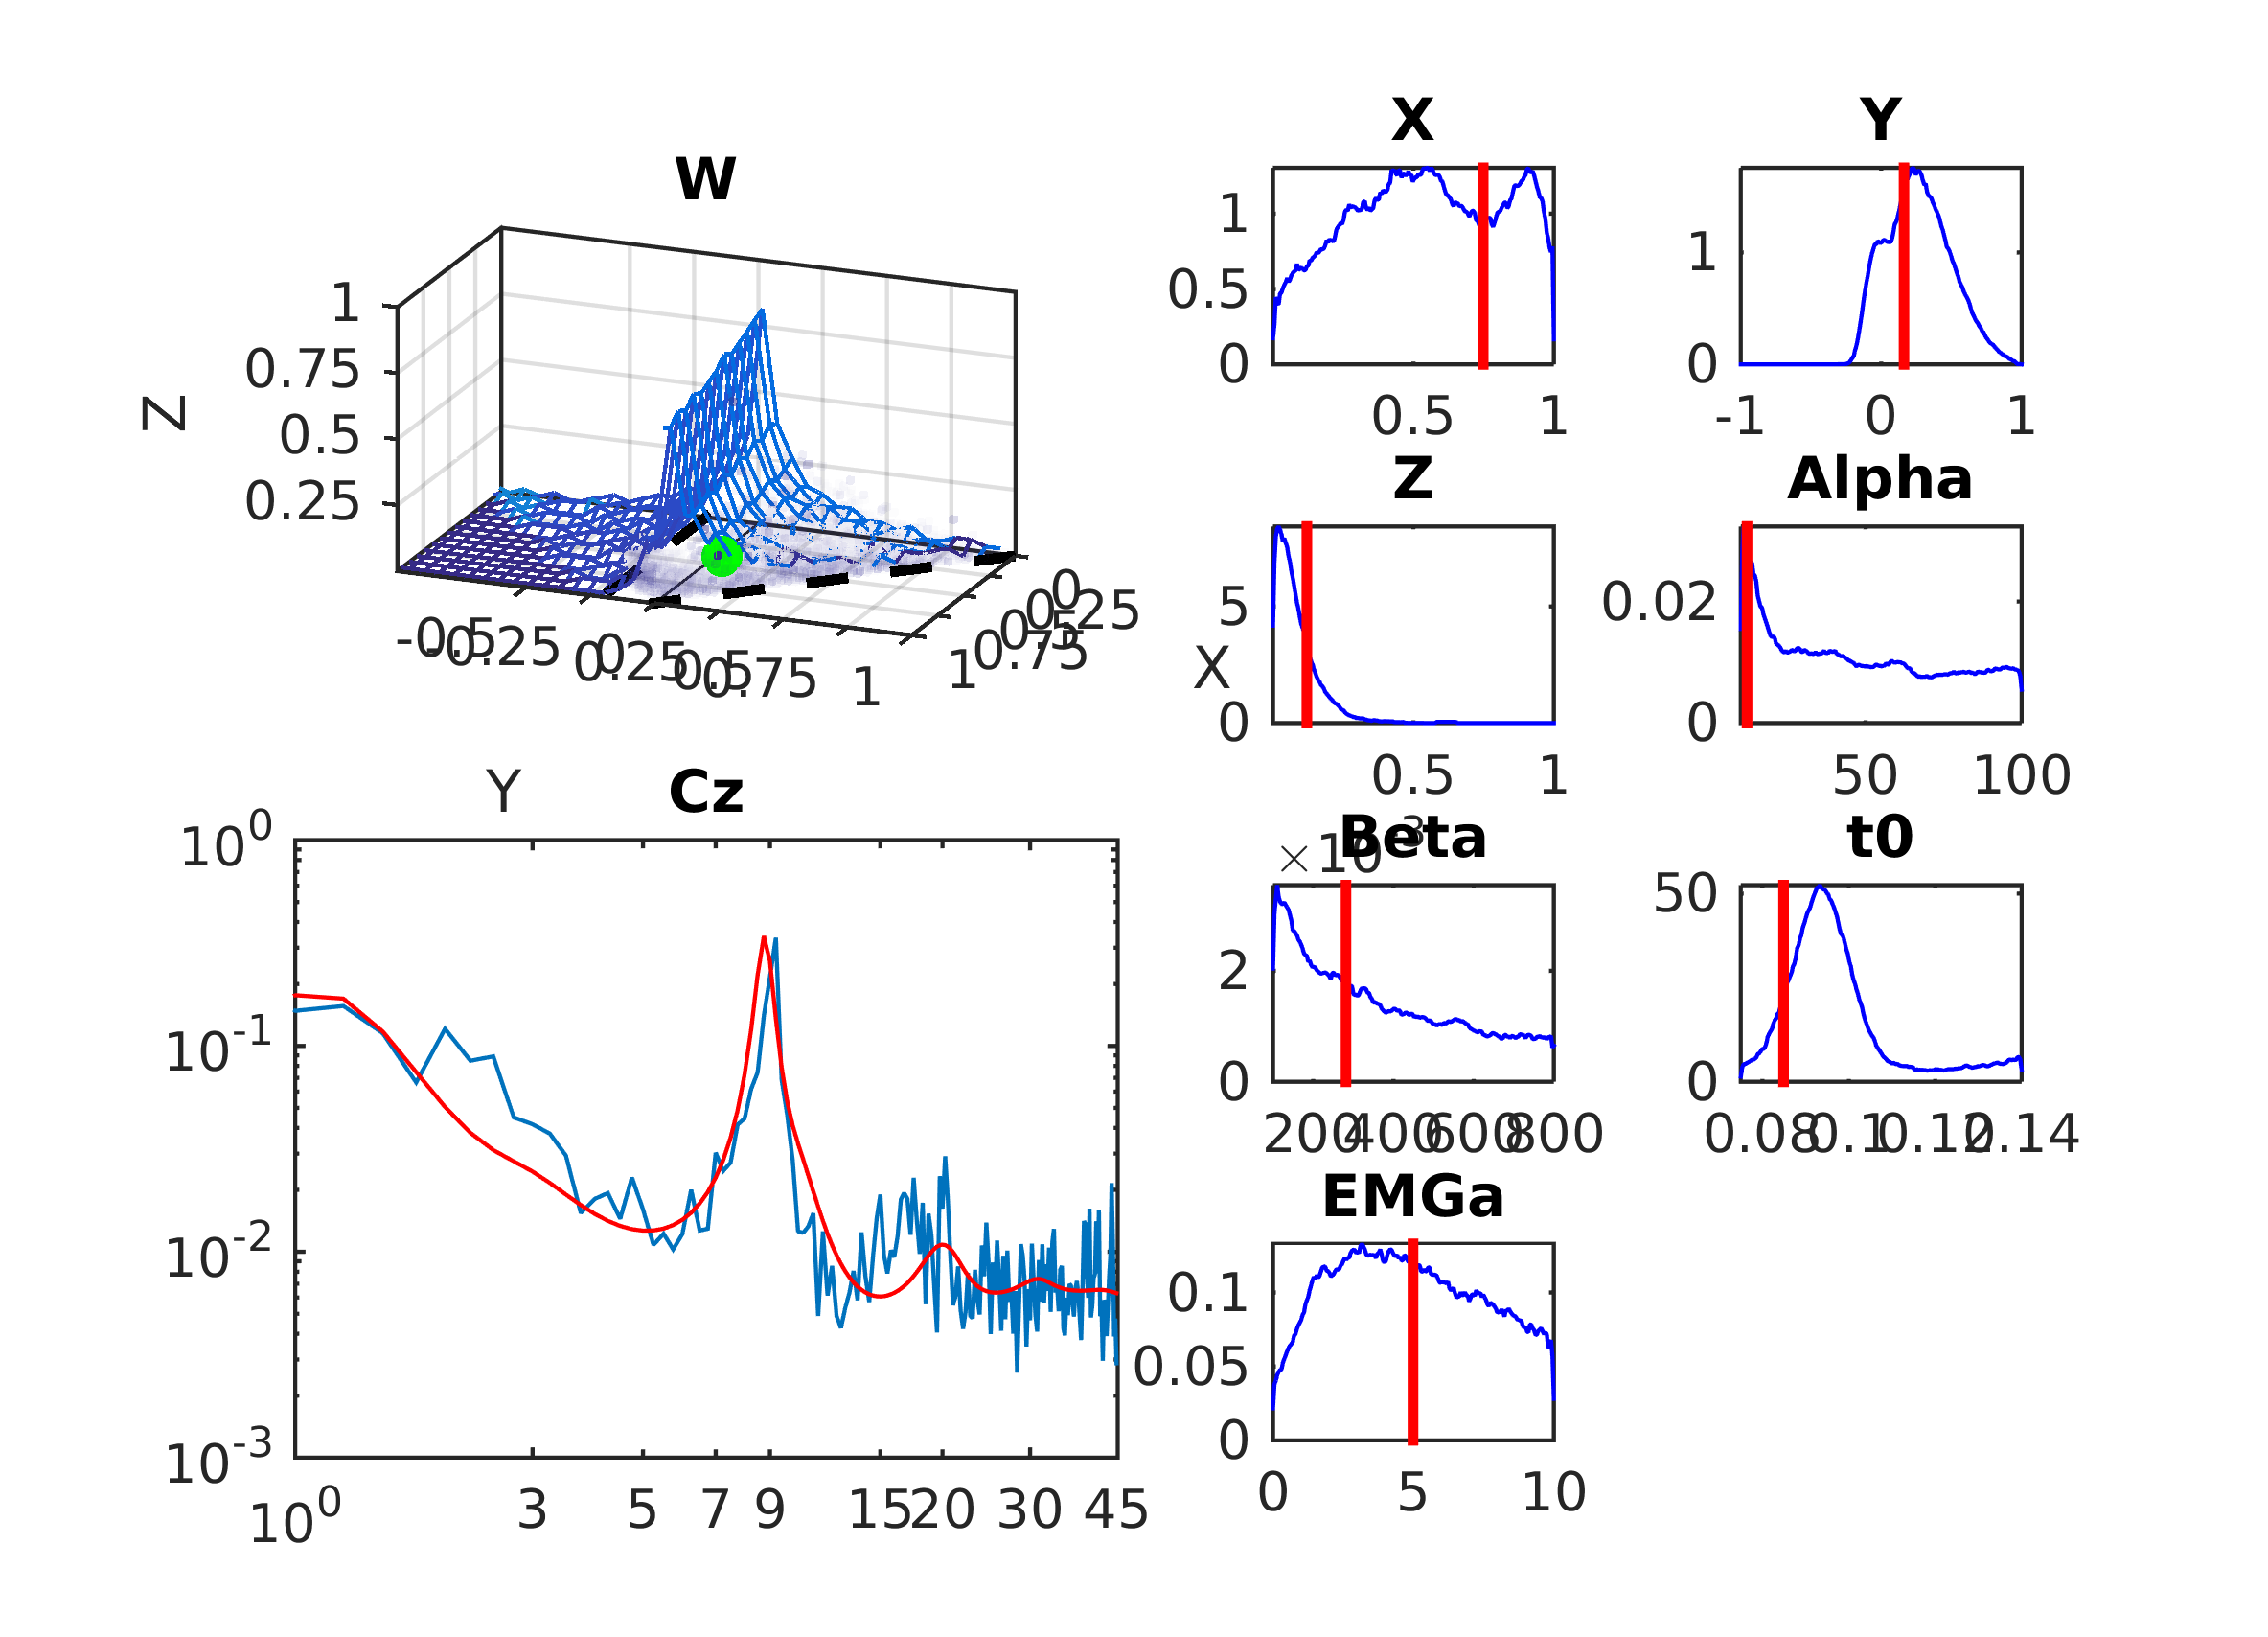
\includegraphics[width=0.8\textwidth]{example_reduced}
\caption{Example fit with reduced model. }
\label{fig:full}
\end{center}
\end{figure}

\clearpage 

\subsection{Reduced model with $L$ in prefactor}
Implemented in {\tt reduced\_ln.m}. This model is the same as \texttt{reduced} except that the factor of $L^2$ is preserved in the prefactor. The power spectrum is then given by:
\begin{align}
	P(\omega) &= \sum_{m = -\infty}^{\infty}\sum_{n = -\infty}^{\infty} P_0 \left| \frac{L^2}{(1+Z'L^2)(k^2r_e^2+q^2r_e^2)}\right|^2,\\[14pt]
\end{align}

\begin{figure}[h!]
\begin{center}
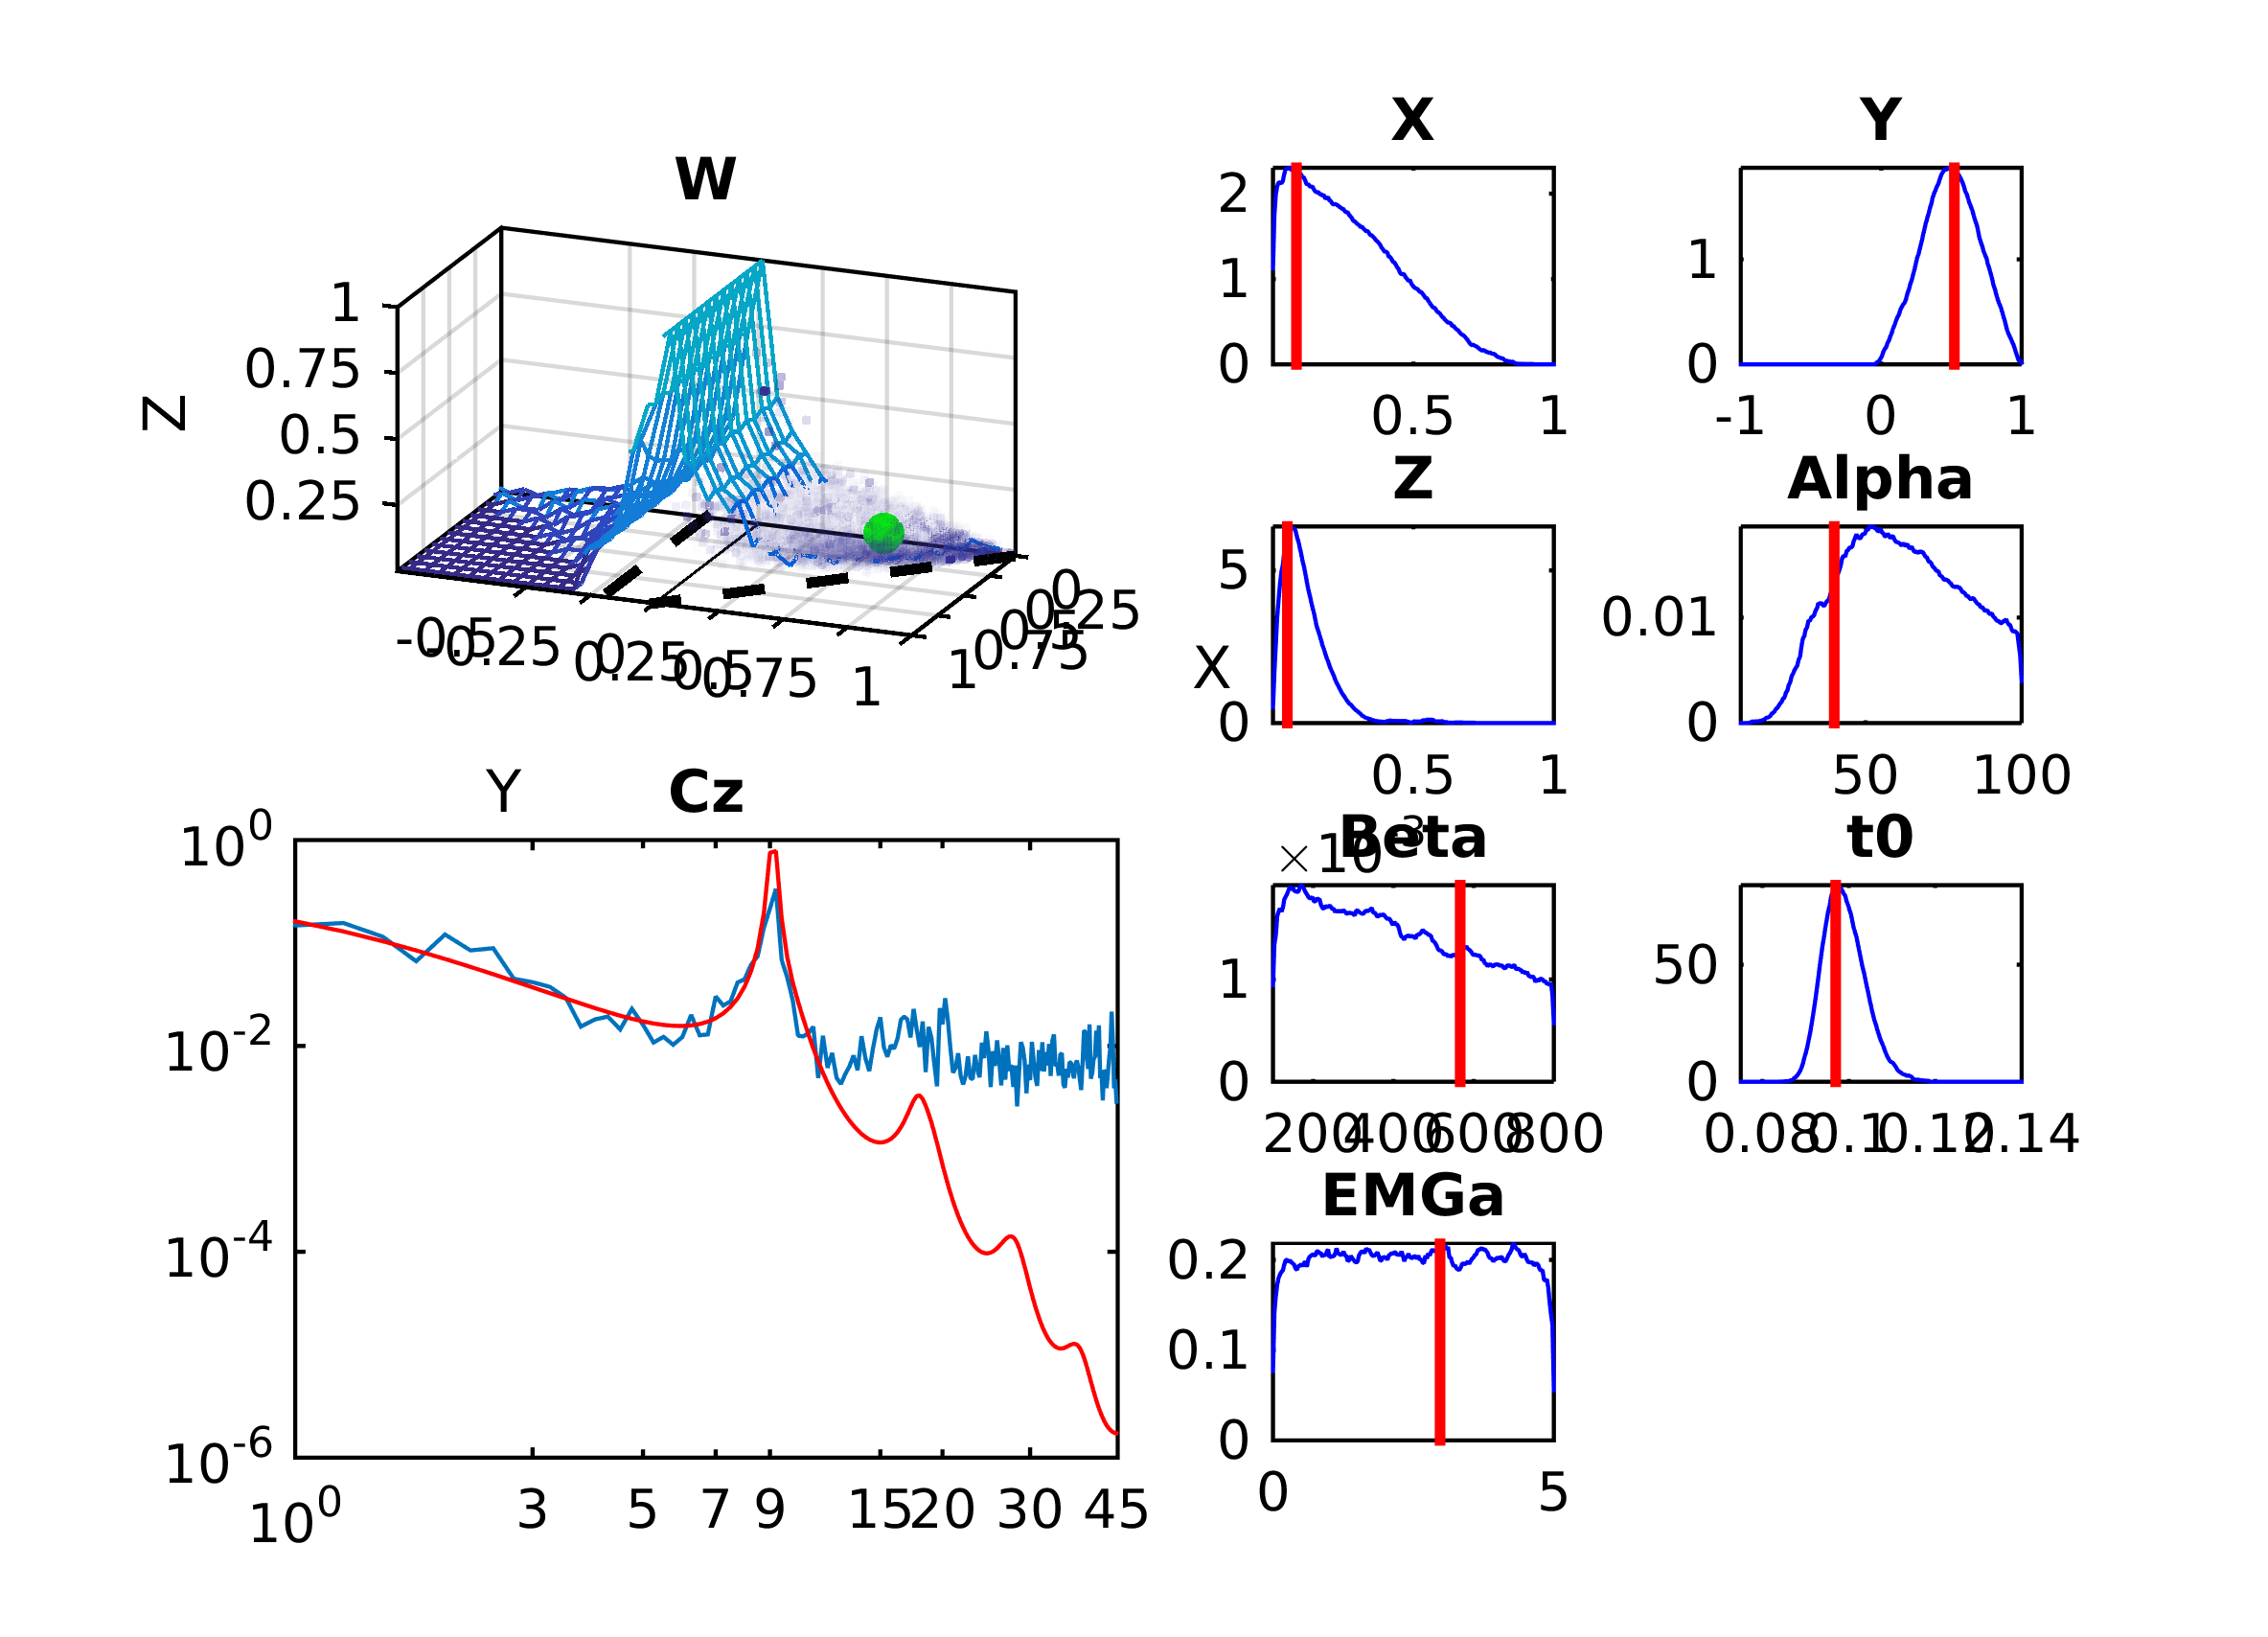
\includegraphics[width=0.8\textwidth]{example_reduced_ln}
\caption{Example fit with reduced model.}
\label{fig:full}
\end{center}
\end{figure}

The primary effect of this modification is to greatly decrease the background power at high frequencies. The harmonic peaks at high frequencies are suppressed a little, but not quite enough. The rolloff at high frequency can be partially fixed with the EMG component but note that the power diverges even for the beta peak, when the EMG component should not have a significant effect.

\begin{figure}[h!]
\begin{center}
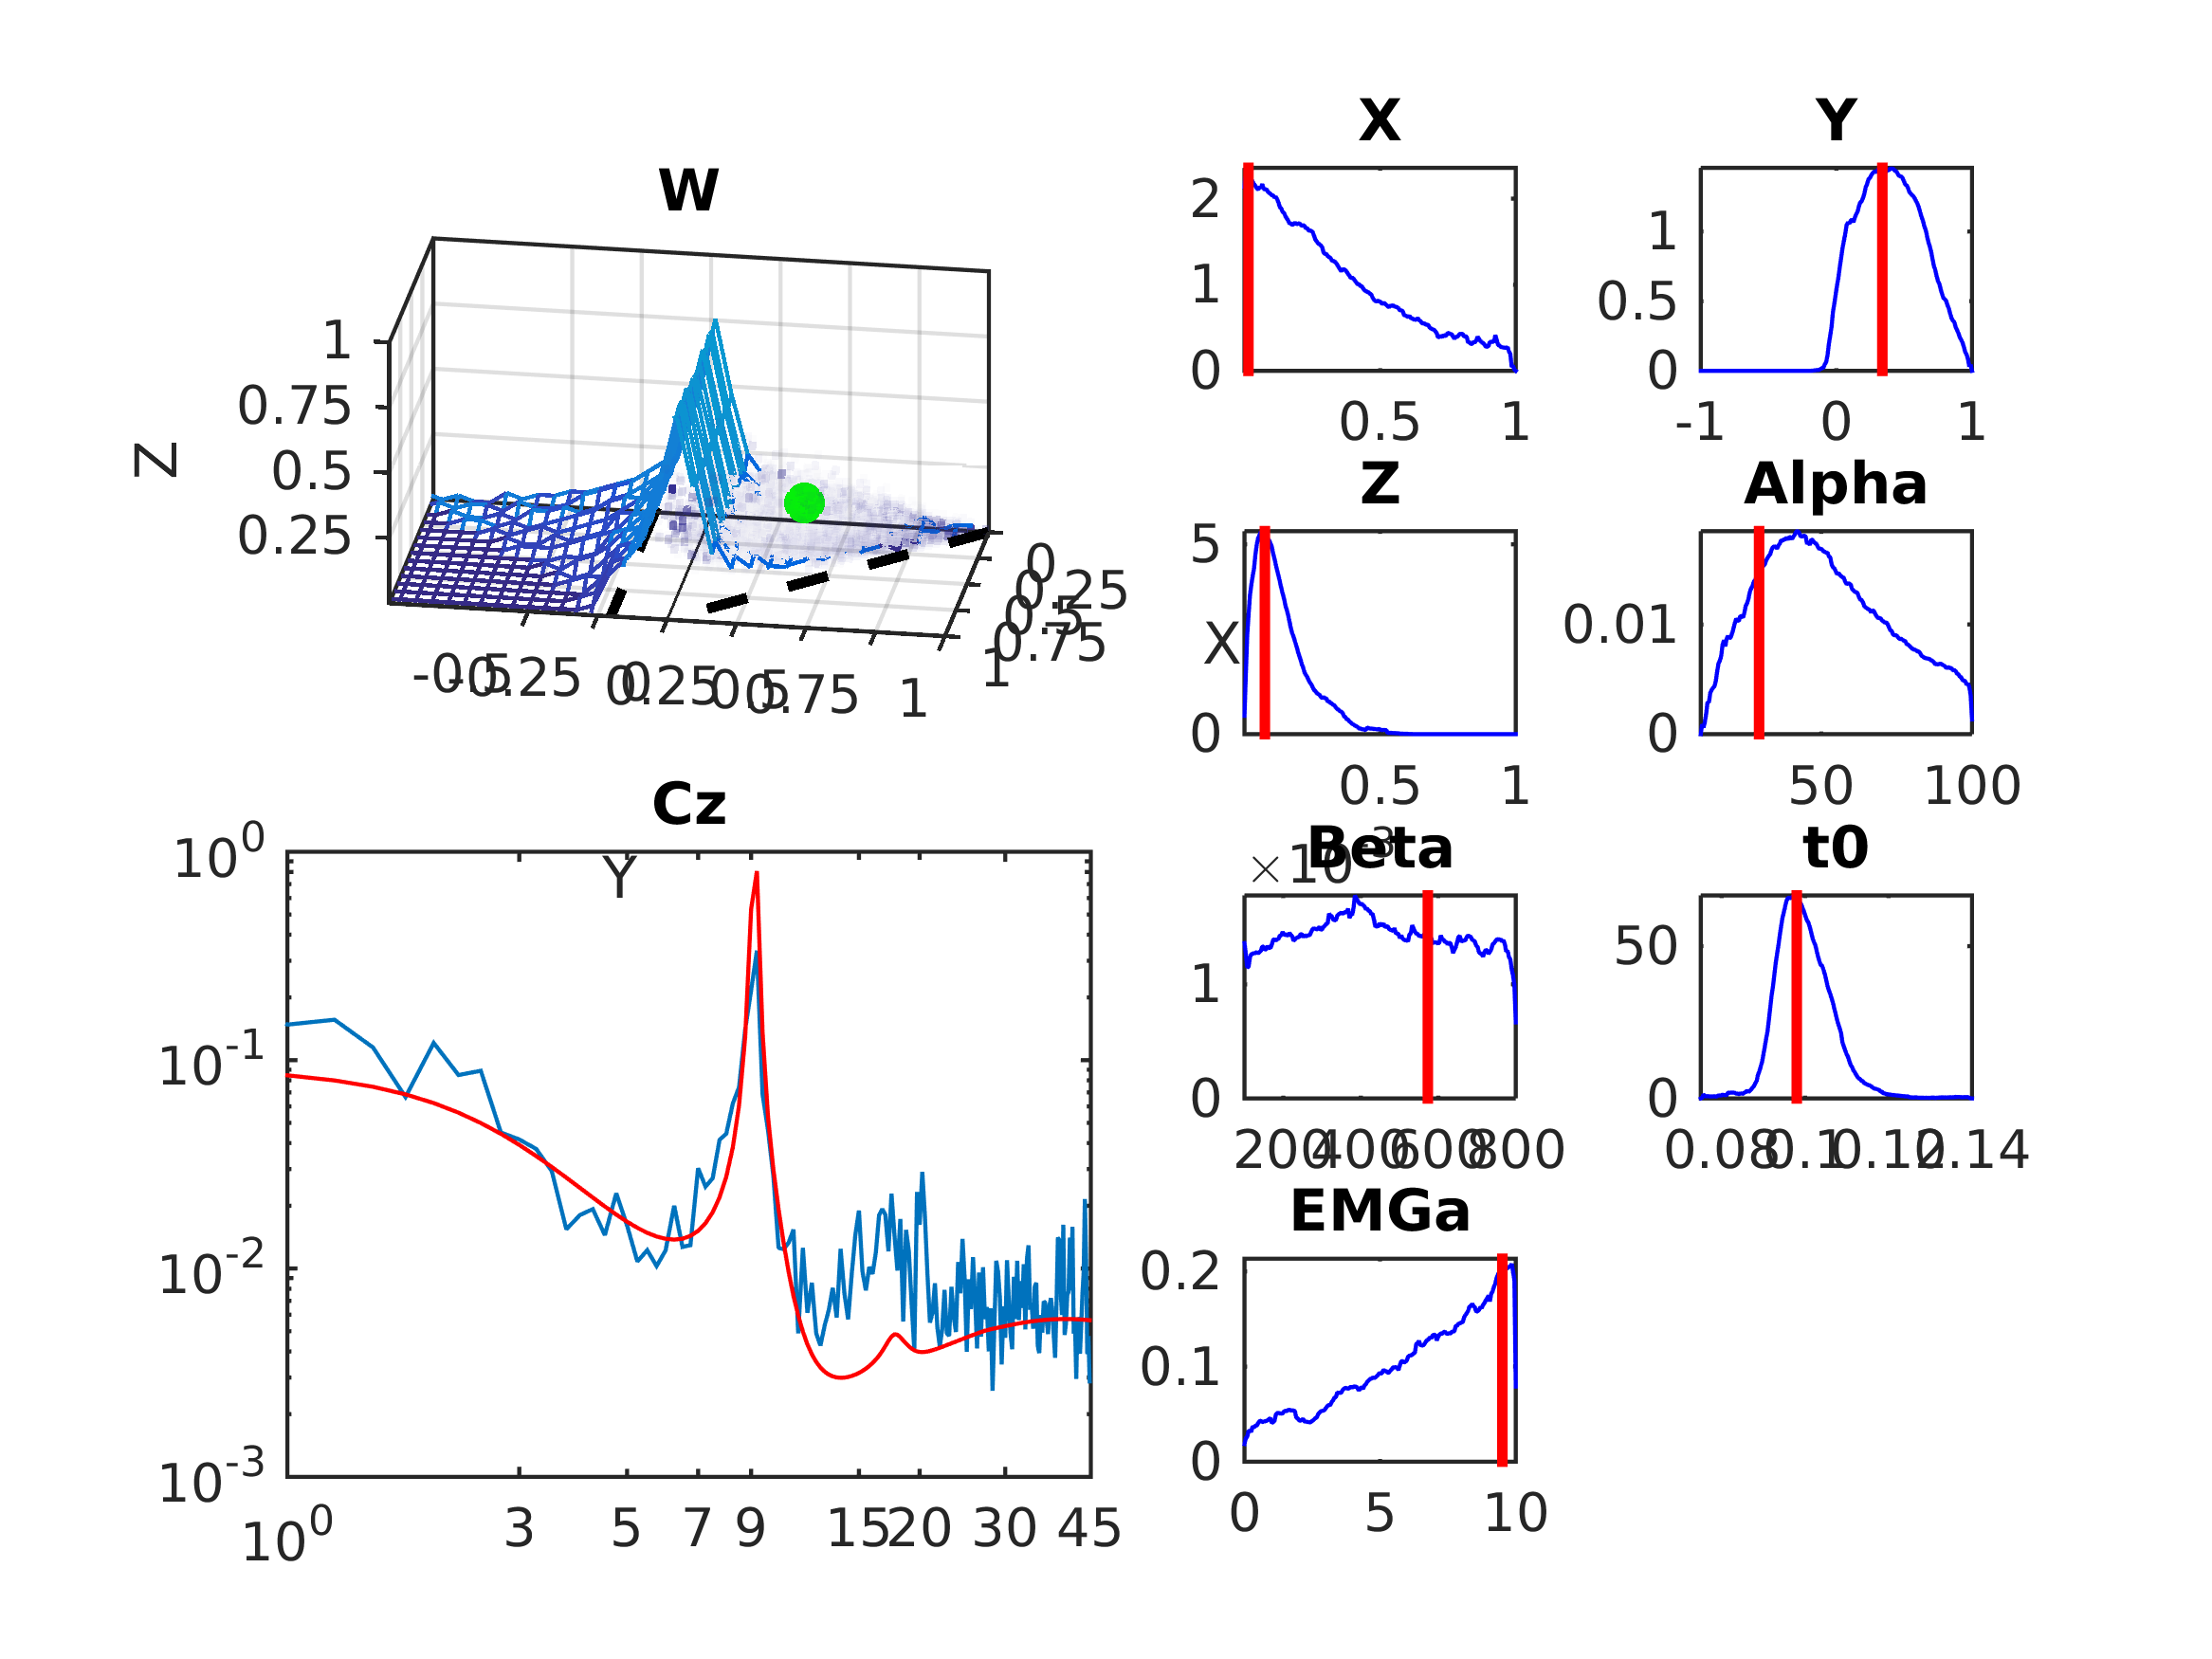
\includegraphics[width=0.8\textwidth]{example_reduced_ln_emg_low}
\caption{Example of \texttt{reduced\_ln} with medium levels of EMG correction. The distribution shows larger values of $A_{EMG}$ may be favored. }
\label{fig:full}
\end{center}
\end{figure}

\begin{figure}[h!]
\begin{center}
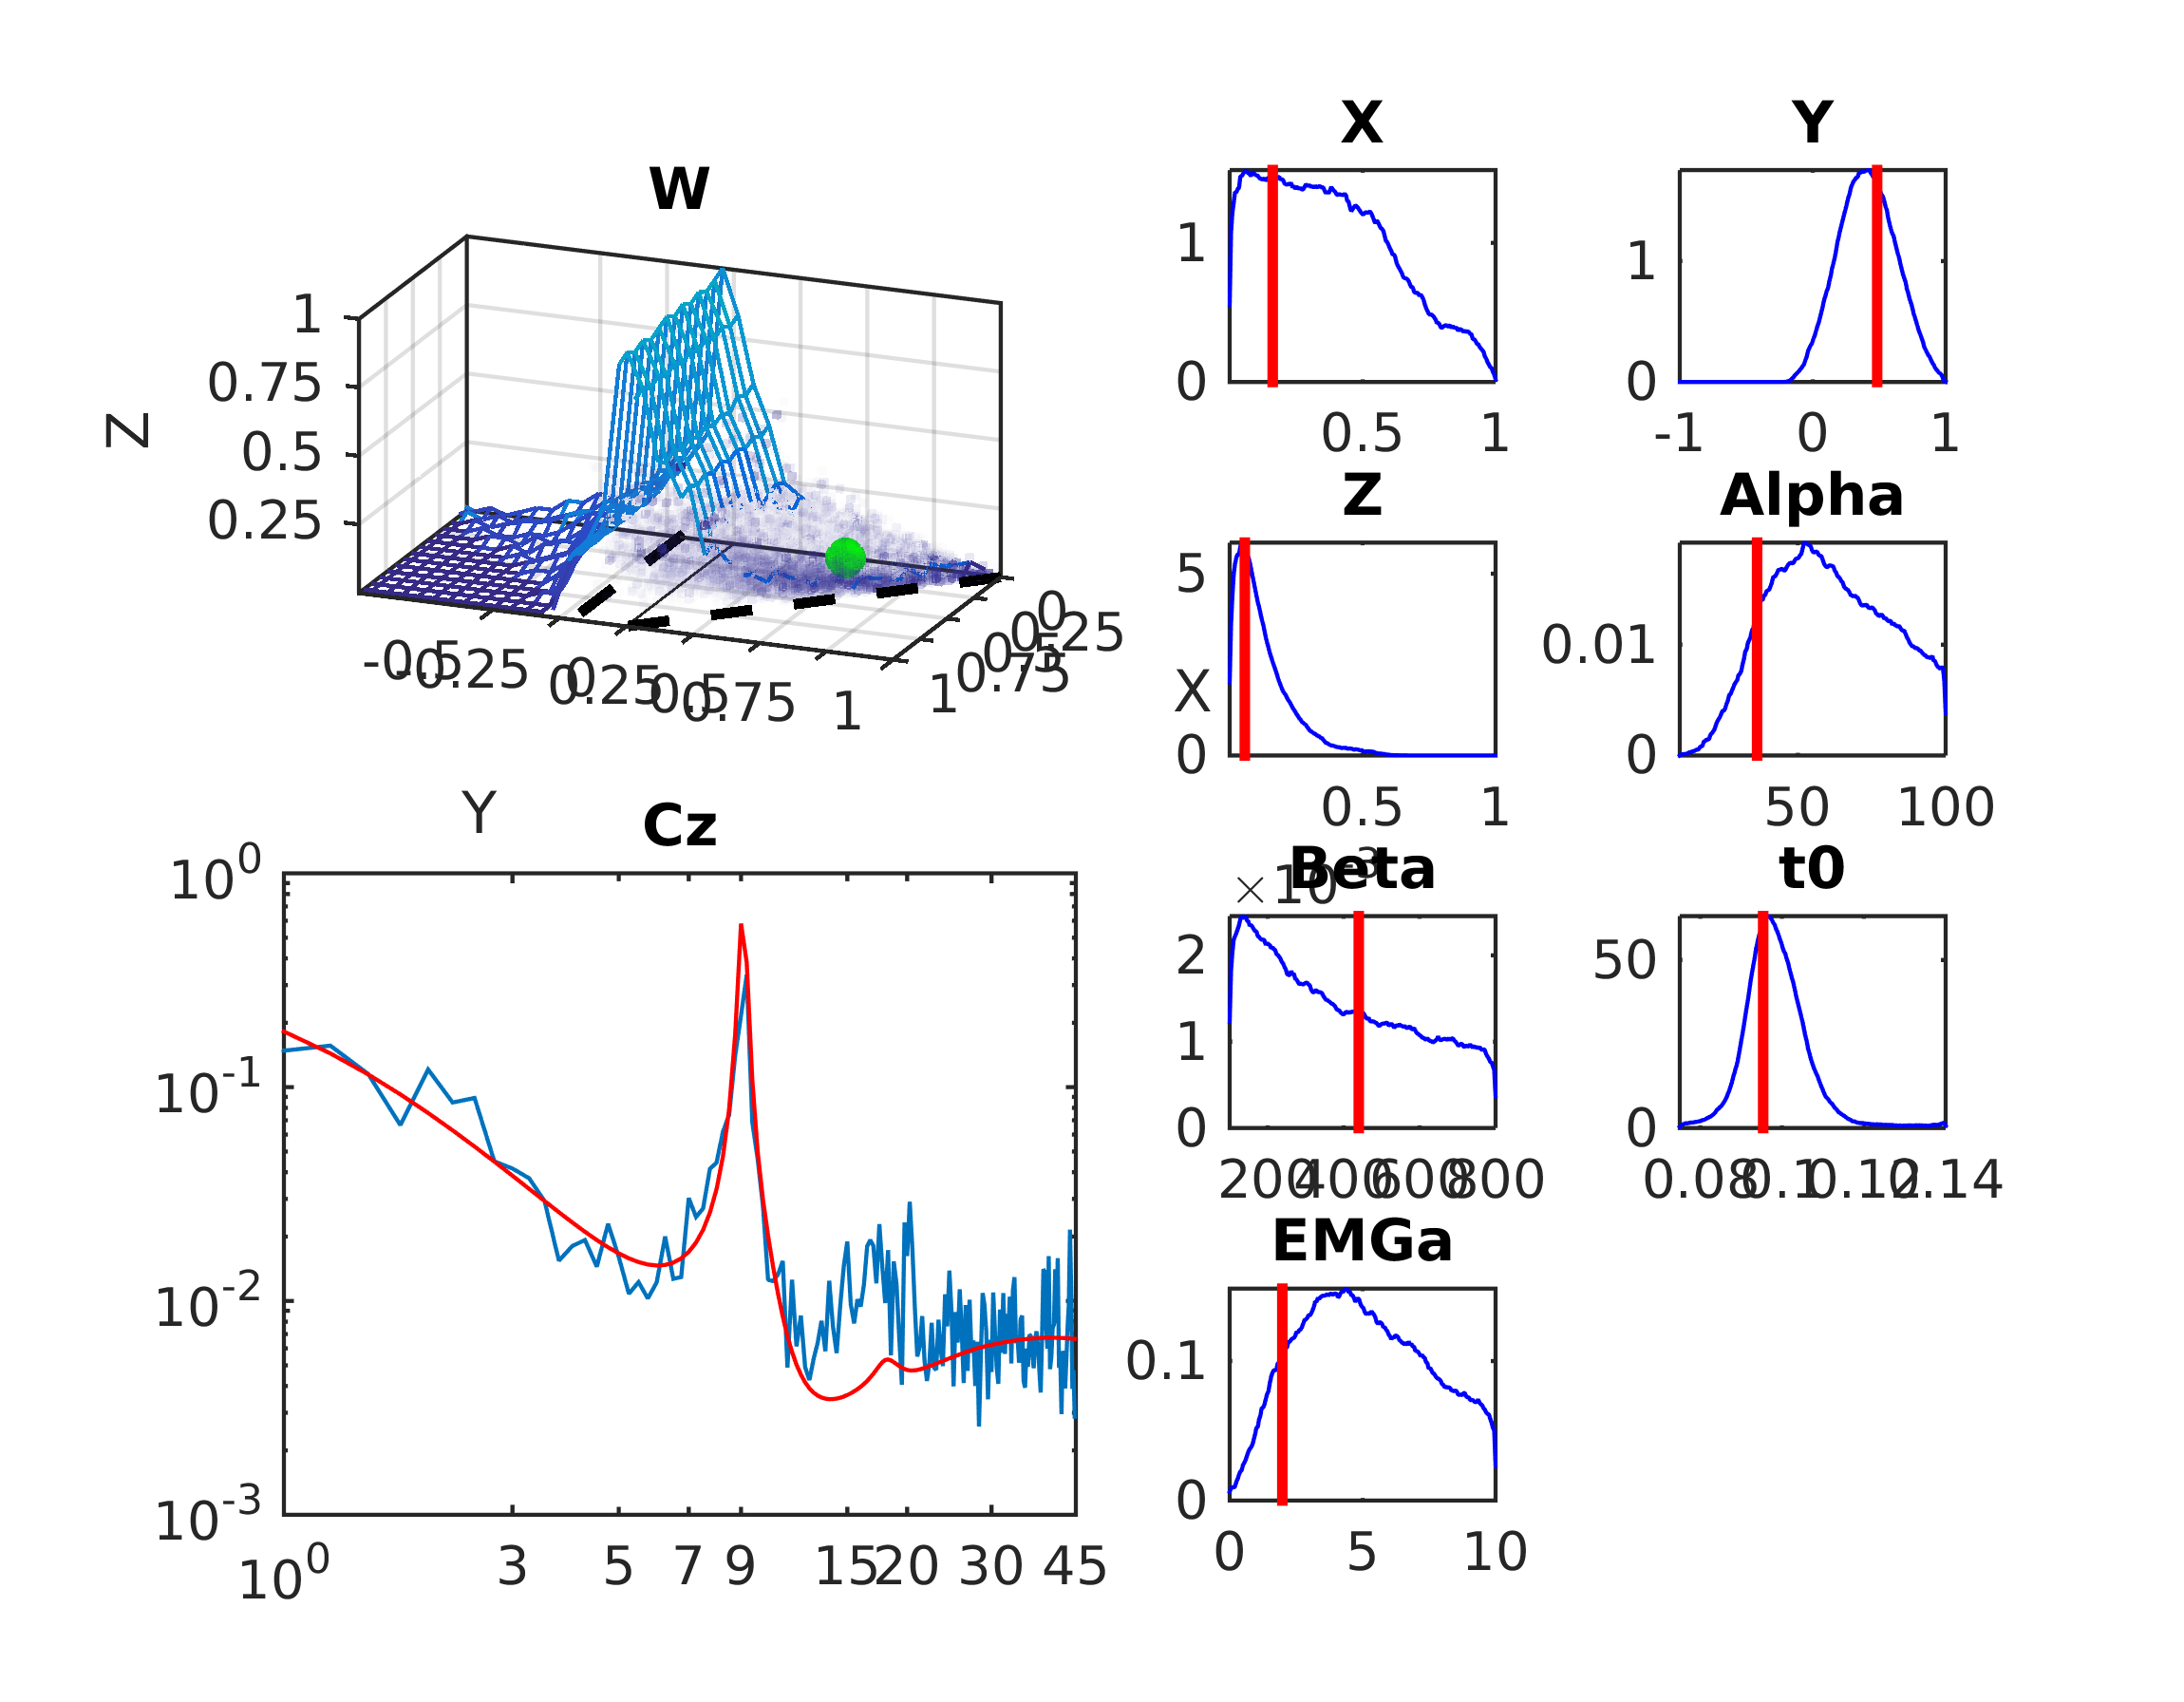
\includegraphics[width=0.8\textwidth]{example_reduced_ln_emg_high}
\caption{Example of \texttt{reduced\_ln} with high levels of EMG correction. The distribution shows an EMG peak, yet the spectrum is still a poor fit near 20\,Hz. }
\label{fig:full}
\end{center}
\end{figure}

\clearpage

\subsection{Reduced model with $L$ in the $Y$ term}
Implemented in {\tt reduced\_ly.m}. Includes EMG. Equations are derived by substituting $L = 1$ into the full model except in $(1-G_{srs}L^2)$. 

\begin{figure}[h!]
\begin{center}
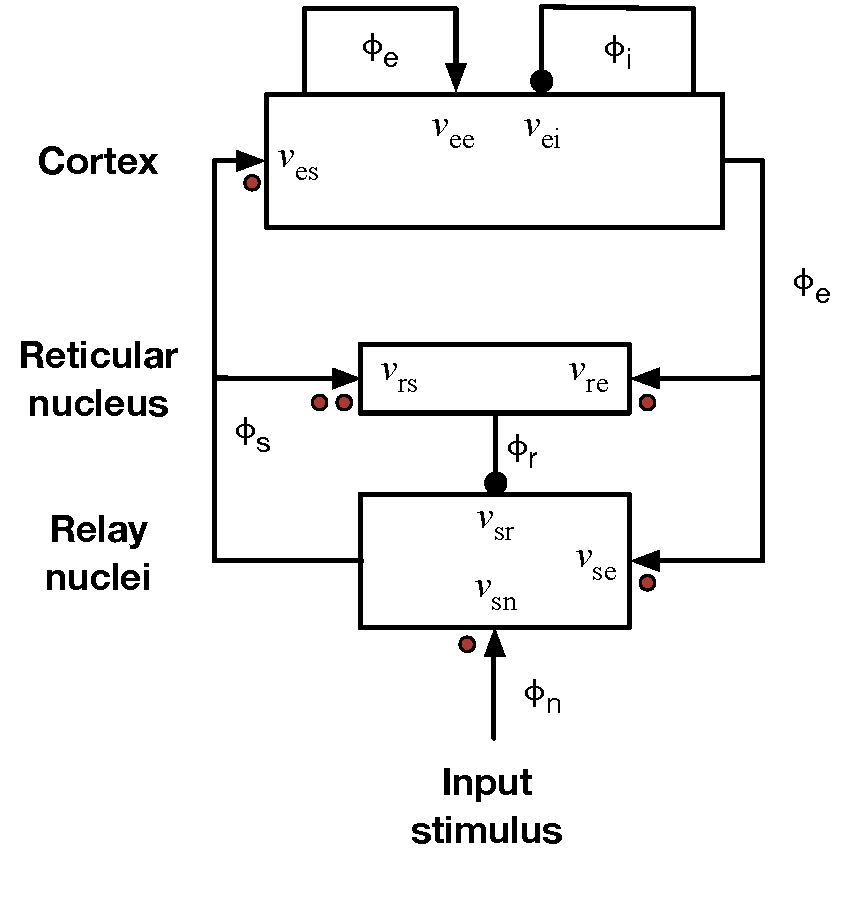
\includegraphics[width=0.4\textwidth]{reduced_ly}
\caption{Reduced model schematic. A factor of $L$ is included for each connection marked with a red dot.}
\label{fig:full}
\end{center}
\end{figure}

Key parameters are $X$, $Y$, $Z$. Stability is given using the dispersion relation
\begin{align}
	\left[ \left(1-\frac{i\omega}{\gamma}\right)^2 - X + k^2r_e^2 \right] \left( 1+Z' L^2 \right) - L^2Y\left( 1+Z' \right) e^{i\omega t_0} &= 0, %JAMES DISPERSION RELATION
\end{align}

with $k=0$. The power spectrum is given by

\begin{align}
	q^2r_e^2 &= \left( 1 - \frac{i \omega}{\gamma}\right)^2  - X - \frac{L^2Y(1+Z')}{1+Z'L^2}e^{i\omega t_0},\\[14pt]
	P(\omega) &= \sum_{m = -\infty}^{\infty}\sum_{n = -\infty}^{\infty} P_0 \left| \frac{L^2}{(1+Z'L^2)(k^2r_e^2+q^2r_e^2)}\right|^2,\\[14pt]
	Z' &= Z \frac{(\alpha+\beta)^2}{\alpha\beta},
\end{align}

\begin{figure}[h!]
\begin{center}
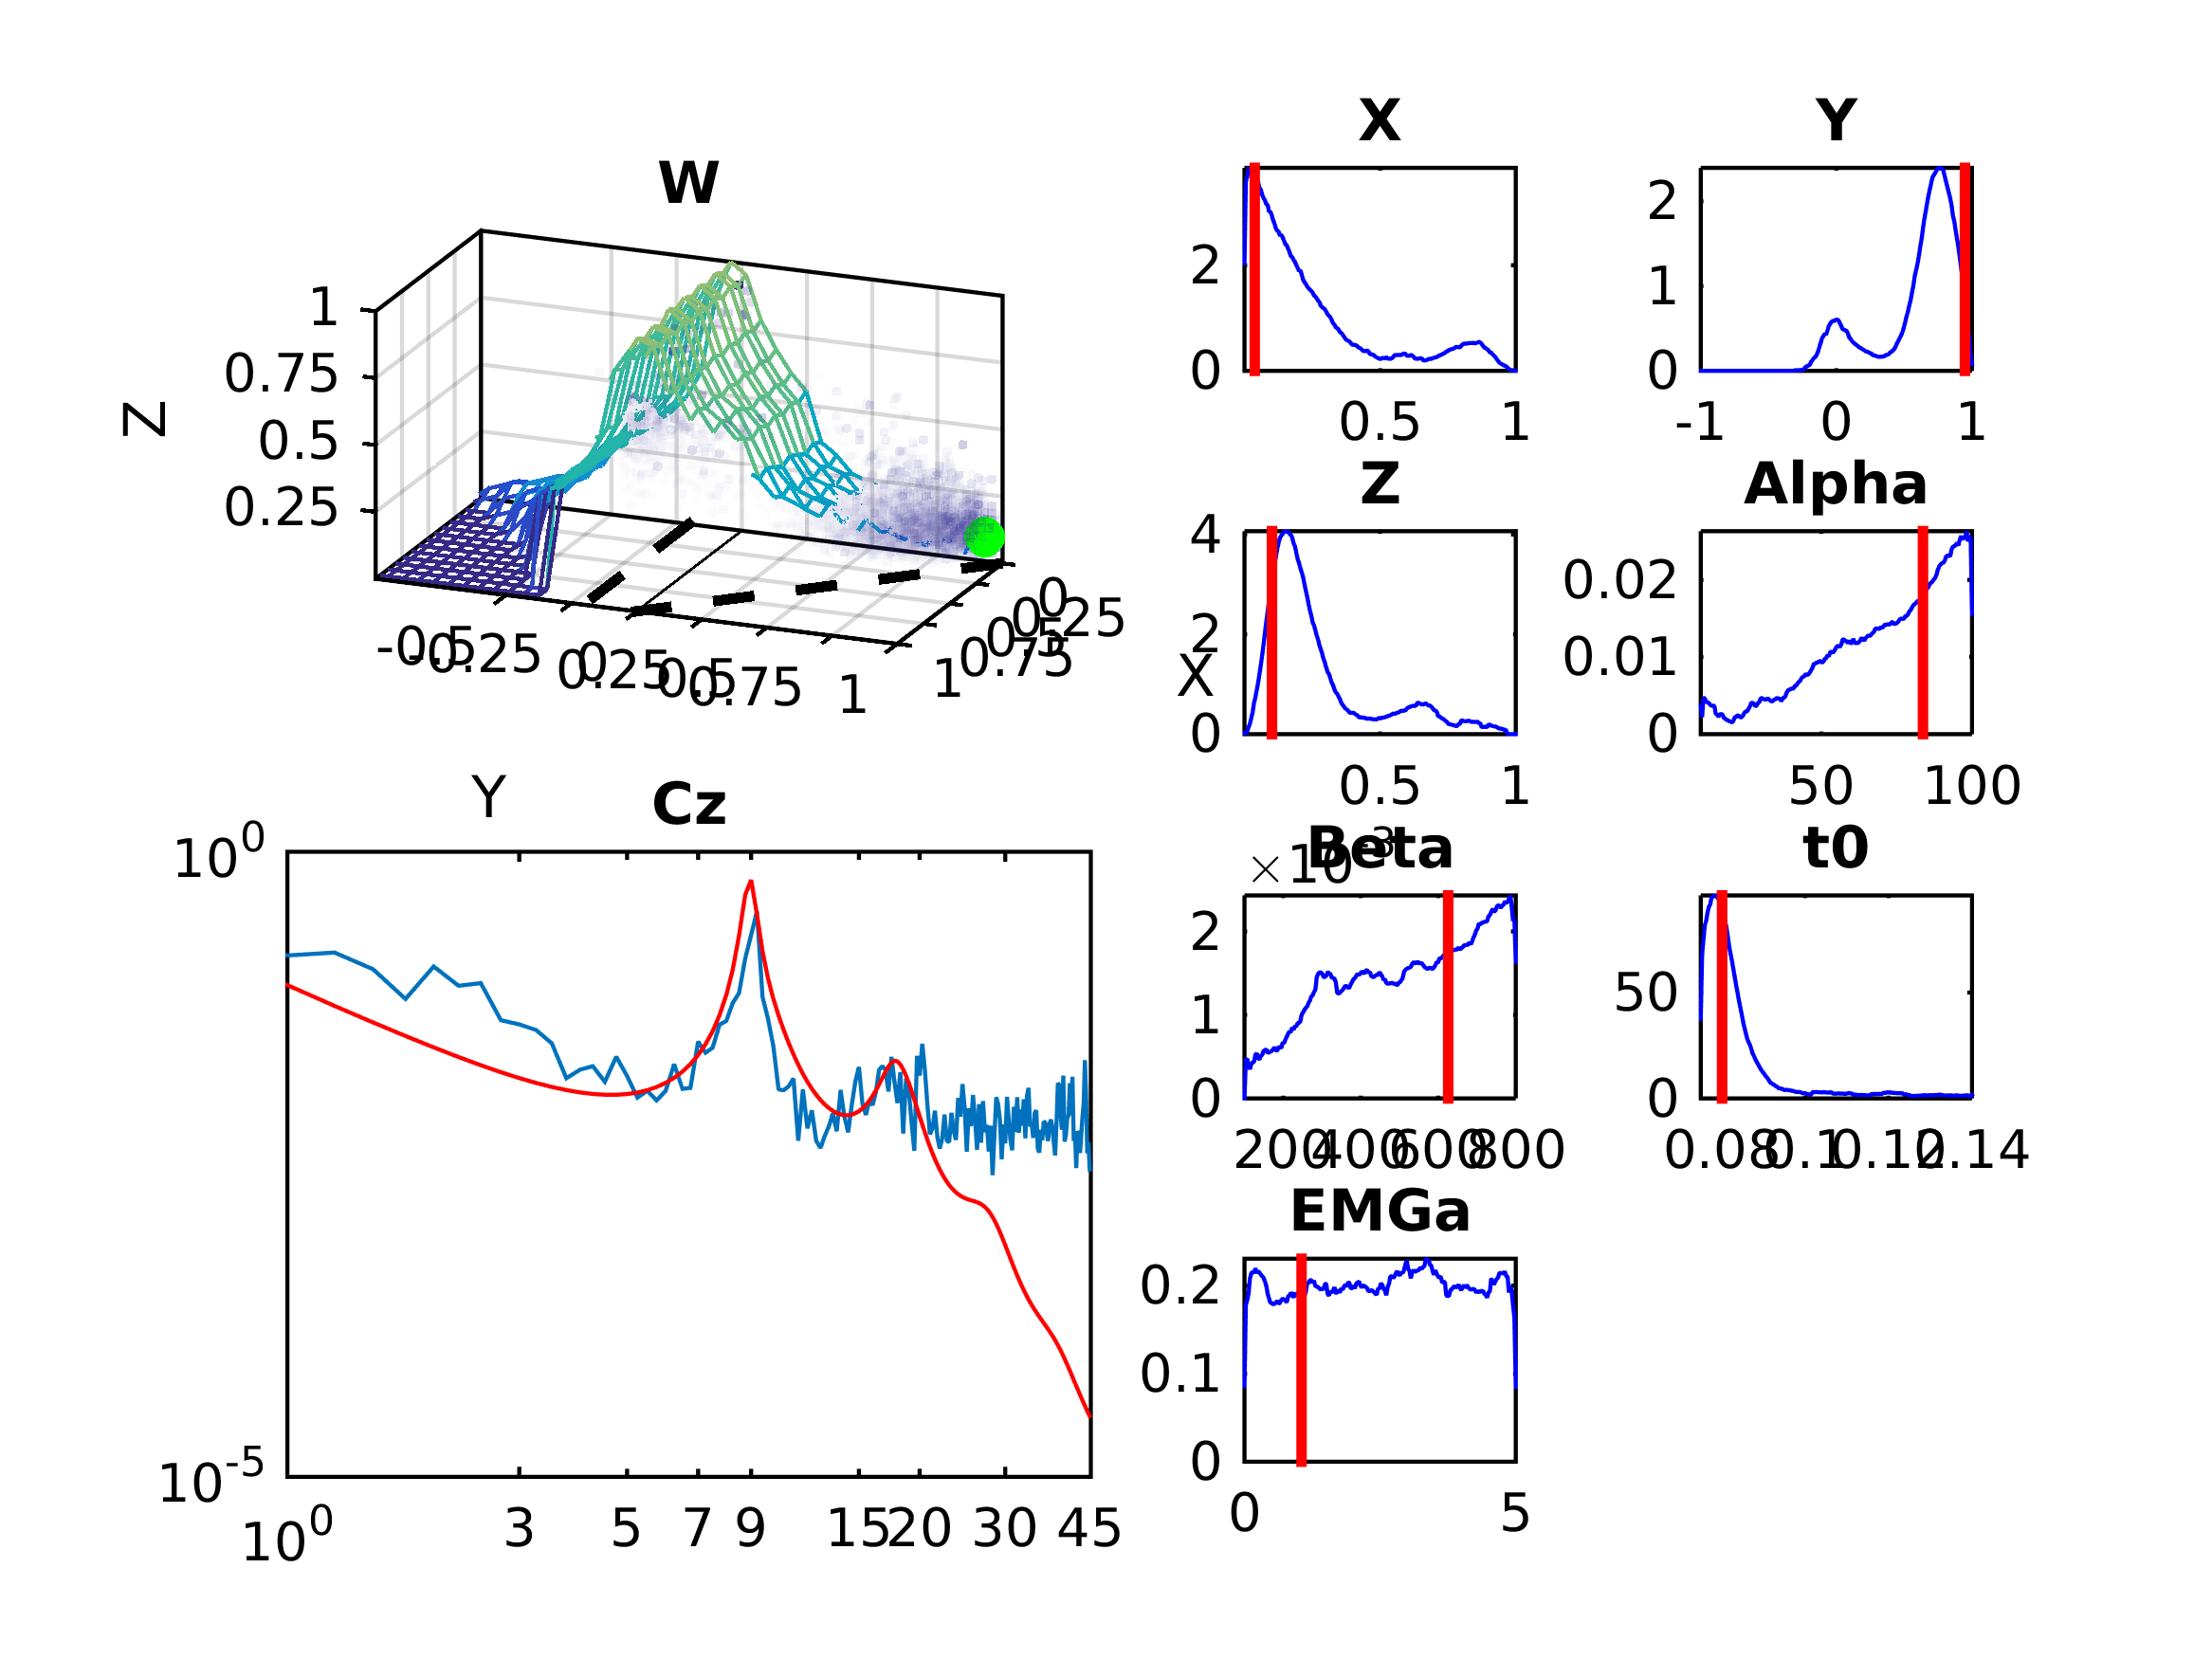
\includegraphics[width=0.8\textwidth]{example_reduced_ly}
\caption{Example fit for \texttt{reduced\_ly}. Note that the stability criteria are now different so the tent surface corresponds to a different model.}
\label{fig:full}
\end{center}
\end{figure}

This model shows good suppression of features at high frequencies but the EMG component is unable to correct the rolloff at high frequencies.


\begin{figure}[h!]
\begin{center}
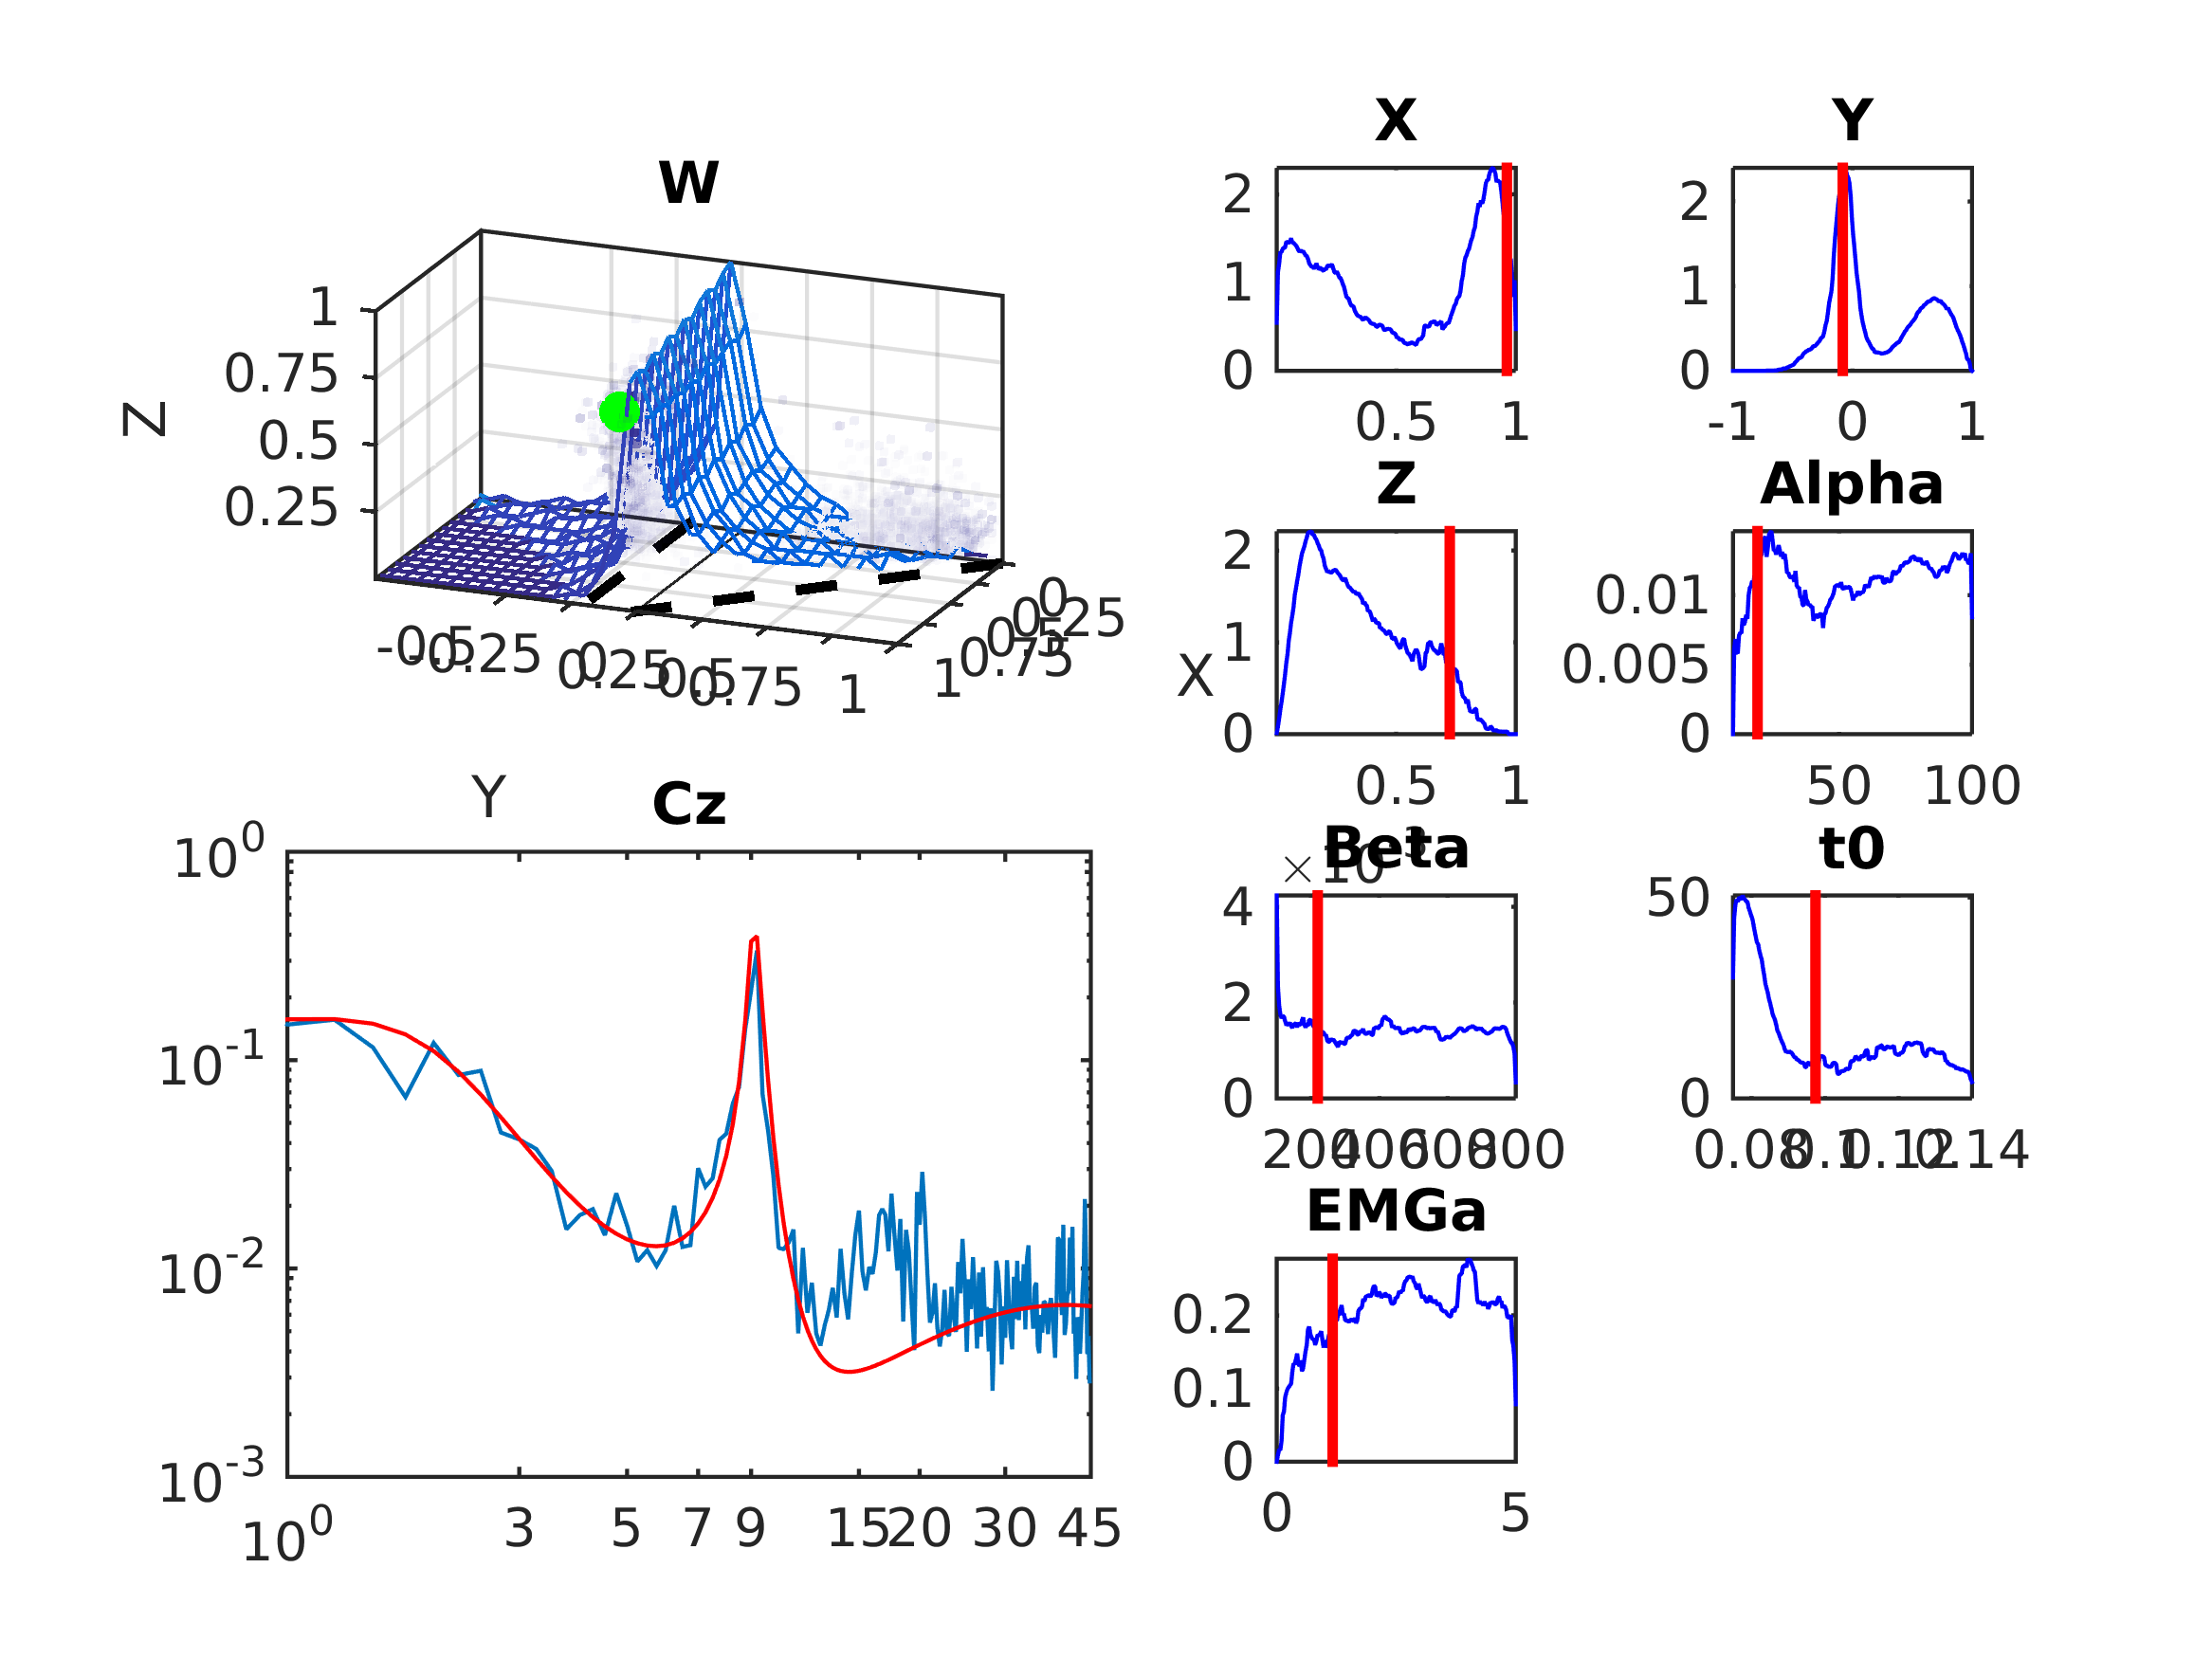
\includegraphics[width=0.8\textwidth]{example_reduced_ly_emg_high}
\caption{Example of \texttt{reduced\_ly} with high levels of EMG correction. Again, the fit at very high frequencies is promoted in favour of discrepencies at lower frequencies.}
\label{fig:full}
\end{center}
\end{figure}


\clearpage

\subsection{Reduced LY with no $L$ prefactor}
Implemented in {\tt reduced\_ly\_no\_n.m}. Includes EMG. The same as \texttt{reduced\_ly} except the $L^2$ is replaced by $1$, the same as in the reduced model i.e.

\begin{align}
	P(\omega) &= \sum_{m = -\infty}^{\infty}\sum_{n = -\infty}^{\infty} P_0 \left| \frac{1}{(1+Z'L^2)(k^2r_e^2+q^2r_e^2)}\right|^2,\\[14pt]
\end{align}

\begin{figure}[h!]
\begin{center}
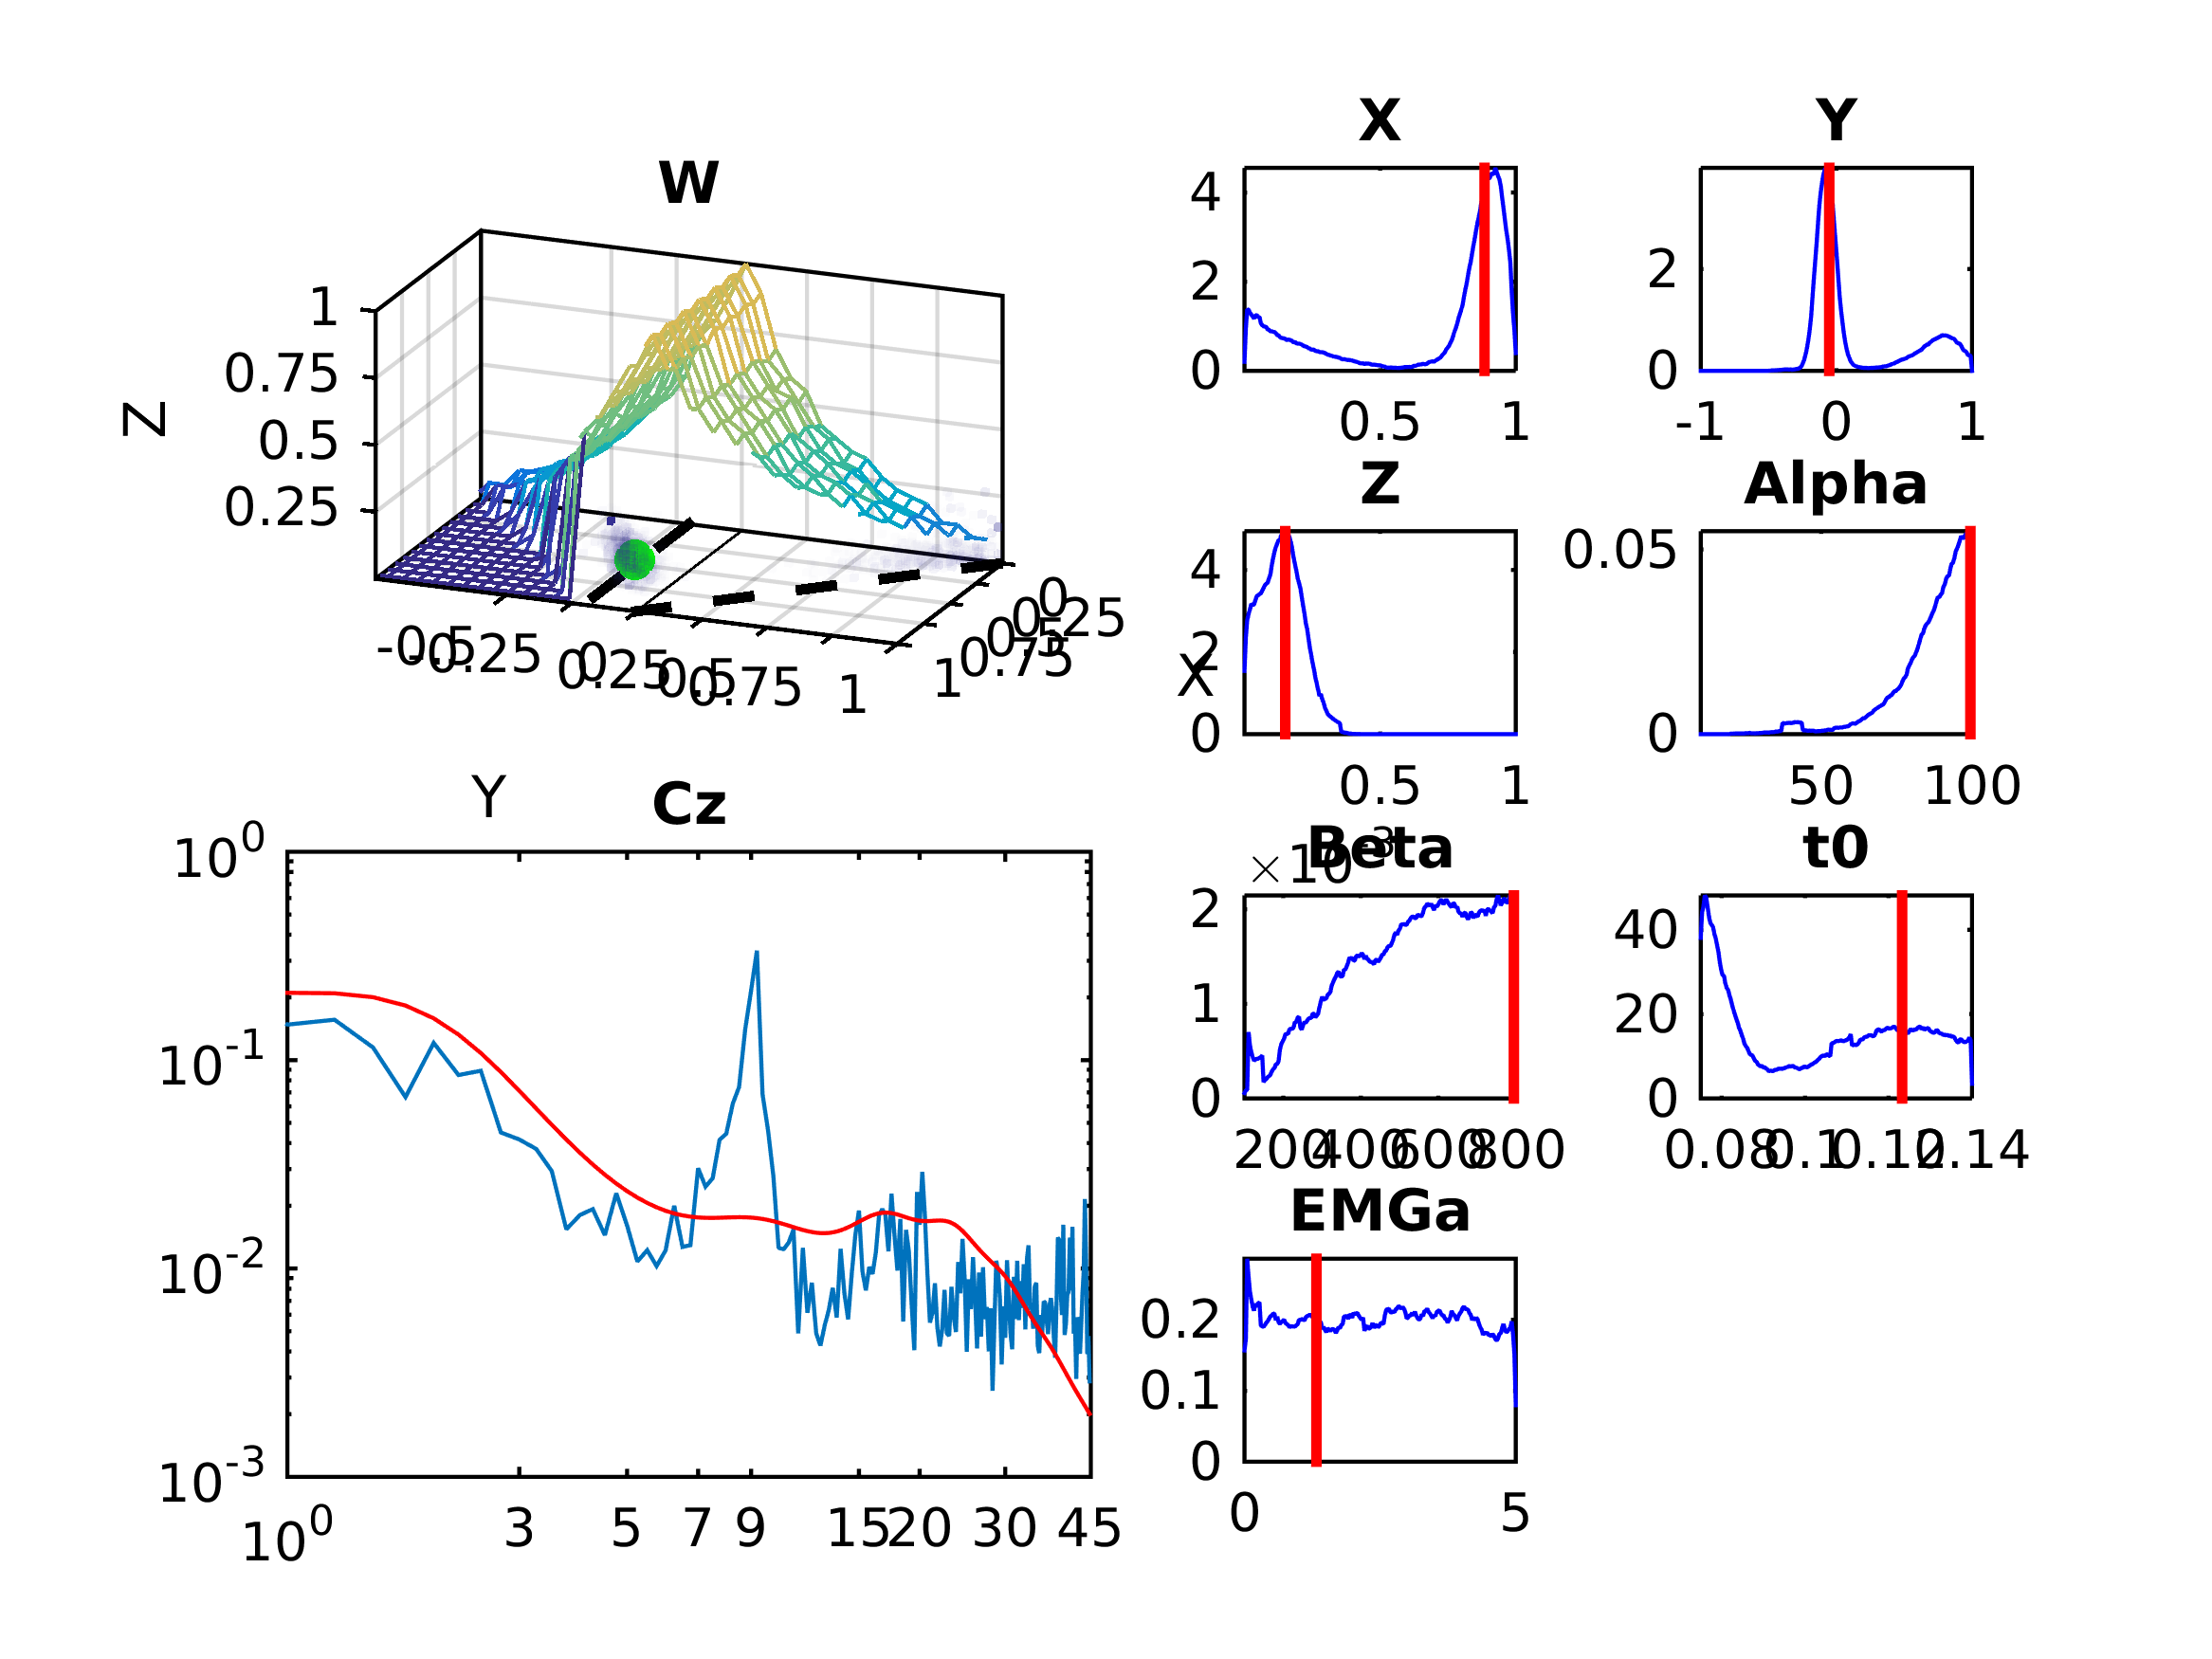
\includegraphics[width=0.8\textwidth]{example_reduced_ly_no_n}
\caption{Example fit \texttt{reduced\_ly\_no\_n}. No EMG component was included (multiplied by 0 internally)}
\label{fig:full}
\end{center}
\end{figure}

This idea didn't seem to work very well. 


\clearpage
\section{Spatial variations}
This program uses a different approach to calculate the power spectrum based on matrix inversion. The model is the same as the full model up to this point: 

\begin{align}
\phi_e \left(D_{e}(1-G_{ei}L) - LG_{ee} - \frac{\left[ L^2G_{ese}  + L^3 G_{erse}\right]e^{i\omega t_0}}{1 - L^2 G_{srs}} \right) &=  \frac{L^2G_{esn}e^{i\omega t_0 /2}\phi_n}{1 - L^2 G_{srs}}\\
\label{spec_spatial}
\phi_e \left(D_{e} - LG_{ee} - \frac{\left[ L^2G_{ese}  + L^3 G_{erse}\right]e^{i\omega t_0}}{(1-G_{ei}L)(1 - L^2 G_{srs})} \right) &=  \frac{L^2G_{esn}e^{i\omega t_0 /2}\phi_n}{(1-G_{ei}L)(1 - L^2 G_{srs})}
\end{align}
where some of the parameters ($G_{ab}$, $t_0$, $L$, others) may depend on position. This equation is of the form
\begin{align}
A(\mathbf{r},\omega) \phi_e(\mathbf{r},\omega) = B(\mathbf{r},\omega) \phi_n(\mathbf{r},\omega)
\end{align}

Taking the Fourier transform of both sides results in a convolution
\begin{align}
A(\mathbf{k},\omega) \ast \phi_e(\mathbf{k},\omega) = B(\mathbf{k},\omega) \ast \phi_n(\mathbf{k},\omega)
\end{align}

Now, the critical step is that any discrete convolution can be written as an equivalent matrix multiplication. This is a nontrivial result. The convolution matrix consists of entries from the original matrix, but rearranged appropriately. The right side of the convolution is reshaped into a column vector, and then the left side of the convolution becomes a square matrix. Each row corresponds to one of the spatial modes. In 1D, the convolution matrix is a circulant matrix. In 2D, the matrix is block circulant. Obtaining the appropriate convolution matrix can be achieved by a very neat result that relates the convolution matrix to the DFT of the identity matrix. In 1D, the arrangement of the convolution matrix can be obtained with

\begin{lstlisting}[style=Matlab-editor,basicstyle=\mlttfamily]
Q = fft(eye(n_modes))
Lm = fft(1:n_modes)
T = round(Q'*diag(Lm)*Q/numel(Lm))
\end{lstlisting}

In 2D, the convolution matrix can be obtained using the Kronecker product
\begin{lstlisting}[style=Matlab-editor,basicstyle=\mlttfamily]
Qm = fft(eye(n_modes))
Q = kron(Qm,Qm)
Lm = fft2(reshape(1:n_modes^2,[n_modes,n_modes]))
T = round(Q'*diag(Lm(:))*Q/numel(Lm))
\end{lstlisting}

The output from these commands corresponds to the indexes of the original matrix being convolved. Thus the equivalence between convolution and matrix multiplication is established via a command like:

\begin{lstlisting}[style=Matlab-editor,basicstyle=\mlttfamily]
conv(A,phie)
A(T)*phie(:)
\end{lstlisting}

It is most convenient in this case to keep the traditional ordering of the frequency components in the DFT - that is, prior to performing an fftshift. The first entry in the matrices thus corresponds to the zero frequency component, rather than the middle entry.

Finally, the spatial operator in $A$ applies only to spatially uniform modes. Therefore, its' Fourier transform $k^2$ is added to the diagonal of the convolution matrix after it has been generated. It is omitted from $D_e$ when computing $A(\mathbf{r},w)$. \emph{Note that this is the reason why the form \eqref{spec_spatial} is preferred - there is no multiplicative factor on $D_e$ which means that $k^2$ can just be directly added, remembering that the other terms can have more complex spatial and frequency dependence.}

Having obtained the convolution matrices $A_c$ and $B_c$, $\phi_e$ can be obtained by matrix inversion

\begin{align}
\phi_e(\mathbf{k},\omega) = A_c^{-1}B_c\phi_n(\mathbf{k},\omega)
\end{align}

Noting that both $\phi_e$ and $\phi_n$ are arranged as column matrices. They can be reshaped into the original 2D matrices afterwards. 

The spectrum $P(\mathbf{k},\omega)$ can be obtained directly from here. Obtaining $P(\mathbf{r},\omega)$ is somewhat more involved, because it requires averaging over the random phases of the white noise input. It can be obtained by assigning $M = A_c^{-1}B_c$. Then

\begin{align}
P(\mathbf{r},\omega) = |\phi_n(\omega)^2| \sum_{\mu,\nu} \exp[i(\mathbf{k}_\mu - \mathbf{k}_\nu) \cdot r] MM\dag
\end{align}

where $\mu$ and $\nu$ range over each of the spatial modes present in the calculation. This formula bears a resemblance to a DFT, but it is not identical. One advantage of this formulation is that it can be computed for an arbitrary set of positions. 


\subsection{Spatial variations in  $t_0$ front-to-back}
Implemented in {\tt spatial\_t0\_2d.m}.

This calculation is essentially the same as the uniform full model, except that $t_0$ is allowed to vary with an amplitude up to $\pm t_0$ along the $Y$-direction of the model. The spatial variation is limited to one spatial wavelength (i.e. one complete oscillation).




\end{document}